\documentclass[11pt,a4paper]{article}
\usepackage[margin=1.5cm, bottom=1.5cm, top=1.5cm]{geometry}
\usepackage{graphicx}
\usepackage{booktabs}
\usepackage{tabularx}
\usepackage{amsmath}
\usepackage{float}
\usepackage{caption}
\usepackage{subcaption}
\usepackage{fancyhdr}
\usepackage{titlesec}
\usepackage{parskip}
\usepackage{enumitem}
\usepackage{hyperref}
\usepackage{microtype}
\usepackage{multicol}

\hypersetup{colorlinks=false,pdfborder={0 0 0}}
\setlength{\parskip}{6pt}
\setlength{\parindent}{0pt}
\raggedbottom
\renewcommand{\baselinestretch}{1.08}

\titleformat{\section}{\large\bfseries}{}{0pt}{}
\titleformat{\subsection}{\normalsize\bfseries}{}{0pt}{}
\titlespacing*{\section}{0pt}{10pt}{5pt}
\titlespacing*{\subsection}{0pt}{8pt}{4pt}
\captionsetup{font=small,labelfont=bf,skip=4pt}
\setlist[itemize]{leftmargin=16pt,itemsep=2pt,topsep=2pt}
\setlength{\textfloatsep}{10pt plus 2.0pt minus 4.0pt}
\setlength{\intextsep}{10pt plus 2.0pt minus 4.0pt}

\pagestyle{fancy}
\fancyhf{}
\fancyhead[L]{\small Individual Project Report}
\fancyhead[R]{\small Manya Jain | 2024102068}
\fancyfoot[C]{\small \thepage}
\renewcommand{\headrulewidth}{0.4pt}

\begin{document}

\begin{center}
{\Large\bfseries Individual Project}\\[6pt]
{\normalsize Manya Jain \quad 2024102068}
\end{center}
\vspace{6pt}

\section{Phase 1: Data Collection and Tokenizer Construction}

In this project, I built and compared two small language models from scratch to see how different languages and dataset sizes affect training. I trained \textbf{Model H} for Hindi (which has a lot of data available) and \textbf{Model L} for Nepali (which has much less data).

To keep the comparison fair, the two models don't share any training text, vocabularies, or tokenizers. This way, any differences in how well they generate text or learn patterns come entirely from the languages themselves. I wrote everything directly in PyTorch including the web scrapers, tokenizers, attention layers, and training loops without using any pre-trained weights or Hugging Face libraries. 

\textbf{Corpus Construction.} The foundation of this project began with collecting and curating large-scale monolingual corpora of comparable magnitude ($\sim$500M words). Sourcing Hindi data was straightforward, I combined the Sangraha Indic corpus, Hindi Wikipedia, government press releases, movie subtitles, and news archives. In contrast, gathering Nepali at a similar scale posed a significant low-resource challenge. Academic corpora such as IRIIS were too small on their own. To bridge the gap, I wrote targeted scrapers to collect articles from Nepali national news outlets, online literary portals, and digital archives.

\textbf{Data Cleaning.} Web text contains encoding errors, boilerplate, and mixed-script debris. I built a unified preprocessing cleaning pipeline that normalized text to Unicode NFC, filtered out lines with low Devanagari character purity (removing English snippets), and performed exact line-level deduplication to eliminate repeated crawl artifacts. 

\begin{table}[htbp]
\centering
\caption{Corpus splits and exact token counts against the $\sim$500M target requirement}
\begin{tabular}{p{5.5cm}rr}
\toprule
\textbf{Metric} & \textbf{Hindi (Model H)} & \textbf{Nepali (Model L)} \\
\midrule
Target training tokens & $\sim$500,000,000 & $\sim$500,000,000 \\
Actual training tokens & 494,479,171 & 556,870,421 \\
Validation tokens & 27,471,065 & 30,937,245 \\
Test tokens & 27,471,065 & 30,937,246 \\
Manual collection portion & 19.9\% & 22.3\% \\
Downloaded portion & 80.1\% & 77.7\% \\
\bottomrule
\end{tabular}
\end{table}

To ensure genuine data collection effort beyond downloading pre-packaged dumps, I tracked a substantial manually scraped component in both languages (19.9\% in Hindi, 22.3\% in Nepali). Rigorous deduplication also prevented crawled snippets from leaking across the evaluation splits.

Each language was partitioned into a deterministic 90/5/5 train, validation, and test split. Although both final corpora reached similar post-cleaning volumes, their underlying domain diversity differs fundamentally. Hindi represents a rich mixture of conversational, journalistic, and literary registers. Nepali is heavily concentrated in formal journalism and archival text. As seen in Phase 2, this qualitative difference in domain variance has a major impact on pretraining loss and generative diversity.

\subsection{Tokenizer Training}

Having prepared the cleaned corpora, I trained custom Byte-Pair Encoding (BPE) tokenizers from scratch for each language. Because standard BPE implementations attempt to load the entire text into RAM (which is impossible for 500M-word corpora on standard compute), I implemented a memory-efficient streaming BPE trainer. The algorithm processes text in streaming chunks, tracks character pair frequencies with a min-heap, prunes singleton words, and dynamically updates adjacent co-occurrence counts after each merge.

Model H and Model L deliberately use two different BPE variants, chosen from the start of the project as a point of comparison:
\begin{itemize}
\item \textbf{Hindi (Byte-level BPE):} Text is first decomposed into raw UTF-8 bytes before merges are learned (the same approach used by GPT-2). Because every possible byte is representable, this variant can encode any input, including rare symbols or mixed script, with a 0.00\% unknown (UNK) rate. This suits Hindi's larger, more diverse corpus (news, Wikipedia, subtitles), which is more likely to contain irregular characters despite the cleaning pipeline.
\item \textbf{Nepali (Unicode character-level BPE):} Merges are learned directly over Devanagari Unicode codepoints rather than bytes. This keeps the vocabulary file human-readable in the native script and ties each token directly to a valid character, at the cost of a small UNK rate (0.00011\%, or just 7 tokens) on characters missing from the training vocabulary.
\end{itemize}
Training both variants let me directly compare a byte-level and a character-level tokenizer under matched conditions (same script family, same general cleaning pipeline). The trade-off is clear: byte-level BPE guarantees zero UNK at the cost of an unreadable, byte-mapped vocabulary file, while character-level BPE keeps the vocabulary readable but sacrifices absolute coverage.

When preparing for full Transformer pretraining in Phase 2, GPU memory constraints dictated balancing embedding parameter overhead against model depth. At a 32K vocabulary, the embedding matrix alone would consume over 16M parameters (nearly two-thirds of our entire parameter budget). Consequently, both tokenizers were fixed to exactly 16,000 vocabulary size for the pretraining runs. This preserved a healthy fertility rate while keeping the embedding size balanced with the rest of the model.

\begin{table}[htbp]
\centering
\caption{Tokenizer measurements on held-out text at exactly 16,000 vocabulary size}
\begin{tabular}{p{5.0cm}rr}
\toprule
\textbf{Measure} & \textbf{Hindi} & \textbf{Nepali} \\
\midrule
Tokenizer type & Byte-level BPE & Character-level BPE \\
Phase 1 vocabulary size & 16,000 & 16,000 \\
Average characters per token & 4.22 & 5.38 \\
Fertility, tokens per word & 1.2052 & 1.2059 \\
Unknown-token rate & 0.00\% & 0.00011\% \\
\bottomrule
\end{tabular}
\end{table}

Nepali requires a slightly larger number of characters per token (5.38 characters/token vs. 4.22 in Hindi) to reach identical fertility (1.205 tokens/word), reflecting its complex suffixes and postpositions. Finally, the entire training split was pre-tokenized and serialized into flat binary arrays of 16-bit integers, memory-mapped via \texttt{np.memmap} for zero-latency, batch-shuffled streaming into the Phase 2 training loop.

\begin{figure}[htbp]
\centering
\begin{subfigure}[b]{0.48\textwidth}
  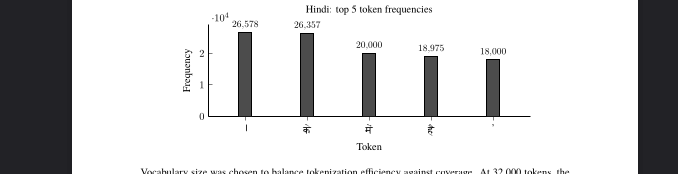
\includegraphics[width=\textwidth]{plots/hindi_freq.png}
\end{subfigure}
\hfill
\begin{subfigure}[b]{0.48\textwidth}
  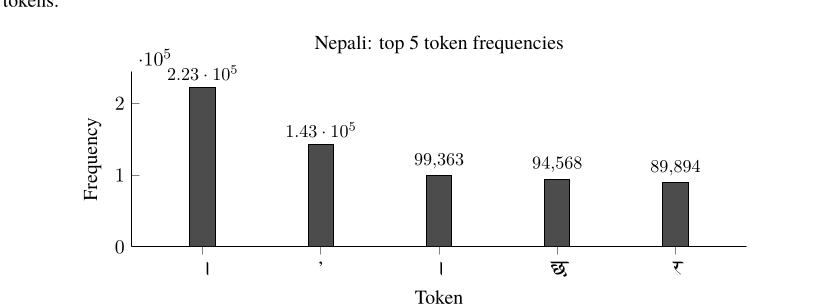
\includegraphics[width=\textwidth]{plots/nepali_freq.png}
\end{subfigure}
\caption{Top 5 token frequencies for Hindi (left) and Nepali (right) showing a Zipfian distribution.}
\end{figure}

\clearpage
\section{Phase 2: Model Implementation and Pretraining}

With memory-mapped token streams ready, I implemented both GPT-style decoder-only Transformer models from scratch in PyTorch. To understand every tensor transformation and gradient flow, I deliberately avoided high-level modules like \texttt{nn.Transformer}. I hand-coded multi-head self-attention, causal masking, learned positional embeddings, layer normalization, and the feed-forward sublayers.

I used a Pre-LayerNorm architecture because it keeps training more stable early on compared to older Post-LN designs. The causal mask prevents tokens from looking ahead at future words by setting the upper-triangular attention scores to negative infinity. Inside the feed-forward network, I used GELU activations and expanded the hidden size to 3 times the model dimension (1,536). I chose learned absolute positional embeddings (constraining max length to 256). I verified the causal mask empirically: modifying token $t+1$ produced exactly 0.0 change in logits at $t$. The dimensions ($d_{model}=512$, 6 layers, 8 heads) were chosen because they keep the parameter count near 25M while remaining wide enough to avoid representation bottlenecks, perfectly fitting the Colab compute budget. The forward pass tensor shapes are: Embeddings (B,T,512) $\rightarrow$ Q/K/V (B,T,512) $\rightarrow$ Split heads (B,8,T,64) $\rightarrow$ Attention output (B,8,T,64) $\rightarrow$ Concatenated (B,T,512) $\rightarrow$ Logits (B,T,16000). Checkpoints saved the model weights, optimizer state, scheduler state, current training step, and configuration. To save parameters and stay under my $\sim$24M limit, I shared the weights between the input embeddings and the final output layer (weight tying).

\begin{table}[htbp]
\centering
\caption{Pretraining architecture and hyperparameter configuration}
\begin{tabular}{p{5.5cm}rr}
\toprule
\textbf{Parameter} & \textbf{Hindi (Model H)} & \textbf{Nepali (Model L)} \\
\midrule
Vocabulary used for pretraining & 16,000 & 16,000 \\
Transformer layers & 6 & 6 \\
Hidden dimension ($d_{model}$) & 512 & 512 \\
Attention heads & 8 & 8 \\
Head dimension ($d_{head}$) & 64 & 64 \\
Feed-forward dimension ($d_{ff}$) & 1,536 & 1,536 \\
Context length & 512 & 512 \\
Dropout rate & 0.1 & 0.1 \\
Total parameters & 24.22M & 24.22M \\
Total pretraining steps & 61,036 & 61,036 \\
\bottomrule
\end{tabular}
\end{table}

Both models were trained using AdamW with a peak learning rate of $5 \times 10^{-4}$, 2,000 steps of linear warmup, and cosine decay down to $10\%$. I engineered a fully resumable checkpointing system that periodically serialized the complete training state, allowing training to recover from transient node interruptions. Both models completed their 61,036-step training schedule stably without divergence, producing two fully trained base language models ready for comparative evaluation.

\subsection{Language-Model Results}

Both pretraining runs exhibited smooth, steady drop in loss. To evaluate generalization, I computed test loss, perplexity ($\mathrm{PPL} = e^{\mathrm{loss}}$), and Bits Per Byte ($\mathrm{BPB} = \frac{\mathrm{loss} \cdot \log_2 e}{\text{bytes per token}}$). Evaluating bits per byte is essential here because raw cross-entropy is parameterized over tokens, making direct cross-lingual loss comparisons misleading when tokenizers differ in byte density.

\begin{table}[htbp]
\centering
\caption{Held-out language-model evaluation metrics}
\begin{tabular}{p{5.5cm}rr}
\toprule
\textbf{Evaluation Metric} & \textbf{Hindi (Model H)} & \textbf{Nepali (Model L)} \\
\midrule
Held-out test loss (nats) & 3.666 & 3.592 \\
Perplexity (PPL) & 39.11 & 36.32 \\
Bits per byte (BPB) & 0.513 & 0.394 \\
Average bytes per token & 10.31 & 13.16 \\
Final validation loss (nats) & 3.649 & 3.605 \\
\bottomrule
\end{tabular}
\end{table}

\begin{figure}[htbp]
\centering
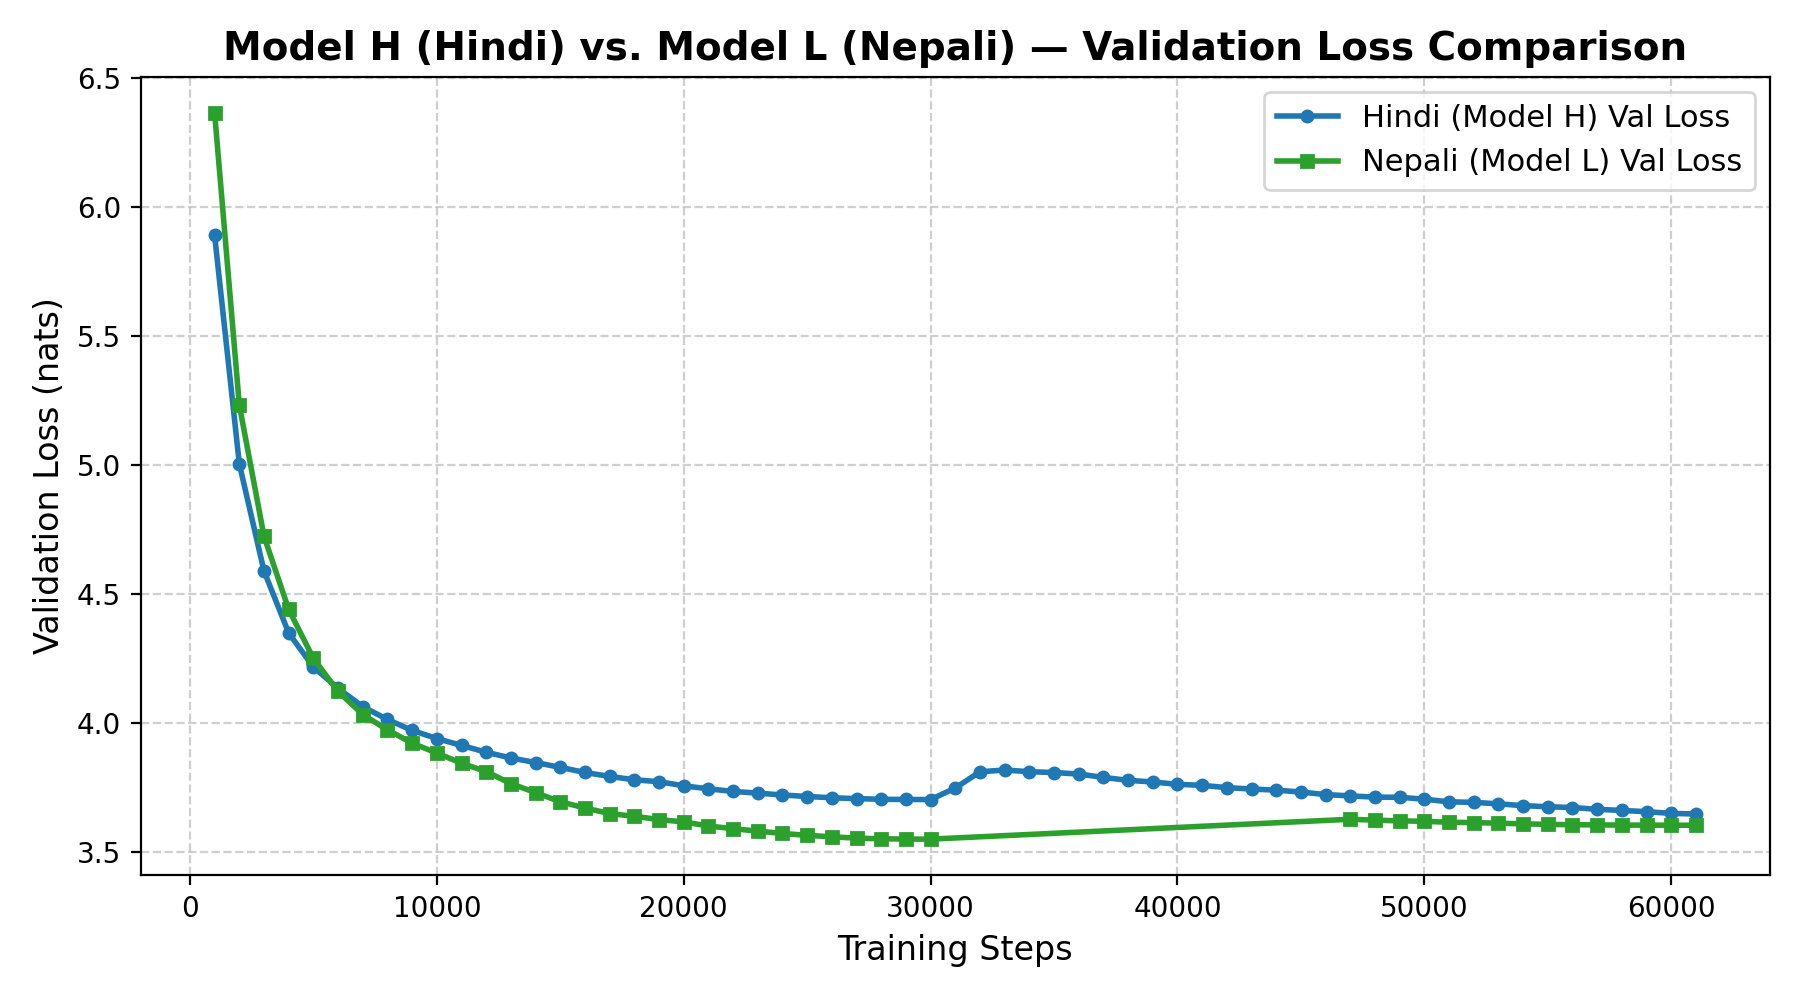
\includegraphics[width=0.95\textwidth]{plots/phase2_comparison_loss_curve.png}
\caption{Validation loss trajectory during 61,036 pretraining steps for Model H and Model L.}
\end{figure}

Nepali achieved lower test loss (3.592 vs. 3.666), lower perplexity (36.32 vs. 39.11), and noticeably lower bits per byte (0.394 vs. 0.513 BPB) than Hindi. However, interpreting this as evidence that Nepali is easier to model would be a mistake. Nepali tokens average 13.16 bytes compared to 10.31 bytes in Hindi, which compresses cross-entropy when normalized into BPB. Furthermore, the Nepali corpus is derived predominantly from formal news and archival documents, making it much more predictable than Hindi's diverse colloquial and literary corpus.

\subsection{Generation and Attention Analysis}

To test whether Model L's low loss hid degenerate behavior, I generated continuations using greedy decoding and temperature sampling, measuring vocabulary diversity via distinct $n$-grams. 

\begin{table}[htbp]
\centering
\caption{Generation metrics and diversity (including Temp 1.5 as required)}
\resizebox{\textwidth}{!}{
\begin{tabular}{llrrrrr}
\toprule
\textbf{Decoding} & \textbf{Model} & \textbf{BLEU-4 / chrF / ROUGE-L} & \textbf{4-gram rep.} & \textbf{Distinct-1} & \textbf{Distinct-2} \\
\midrule
Greedy & Hindi (H) & 0.95 / 12.21 / 0.12 & 0.2659 & 0.4270 & 0.6215 \\
Greedy & Nepali (L) & 1.22 / 13.54 / 0.08 & 0.6712 & 0.2291 & 0.3167 \\
Temp 0.5 & Hindi (H) & 0.77 / 13.45 / 0.09 & 0.1012 & 0.4605 & 0.7336 \\
Temp 0.5 & Nepali (L) & 1.56 / 19.88 / 0.10 & 0.3351 & 0.3981 & 0.6283 \\
Temp 1.0 & Hindi (H) & 0.72 / 12.71 / 0.09 & 0.0267 & 0.6838 & 0.9313 \\
Temp 1.0 & Nepali (L) & 1.06 / 19.27 / 0.09 & 0.0213 & 0.7214 & 0.9586 \\
Temp 1.5 & Hindi (H) & 0.00 / 0.00 / 0.00 & 0.0000 & 0.9447 & 1.0000 \\
Temp 1.5 & Nepali (L) & 0.00 / 0.00 / 0.00 & 0.0000 & 0.9079 & 0.9990 \\
\bottomrule
\end{tabular}}
\end{table}



Under greedy decoding, Nepali suffers from repeating the same phrases, repeating 4-grams 67.1\% of the time. Hindi, by contrast, generates far more diverse text (26.6\% repetition). This confirms that Model L's low pretraining loss was a consequence of learning a narrower, repetitive news distribution rather than acquiring deeper linguistic generalization. Temperature sampling ($T=0.5$) successfully broke the repetitive cycles in both models.

\begin{figure}[htbp]
\centering
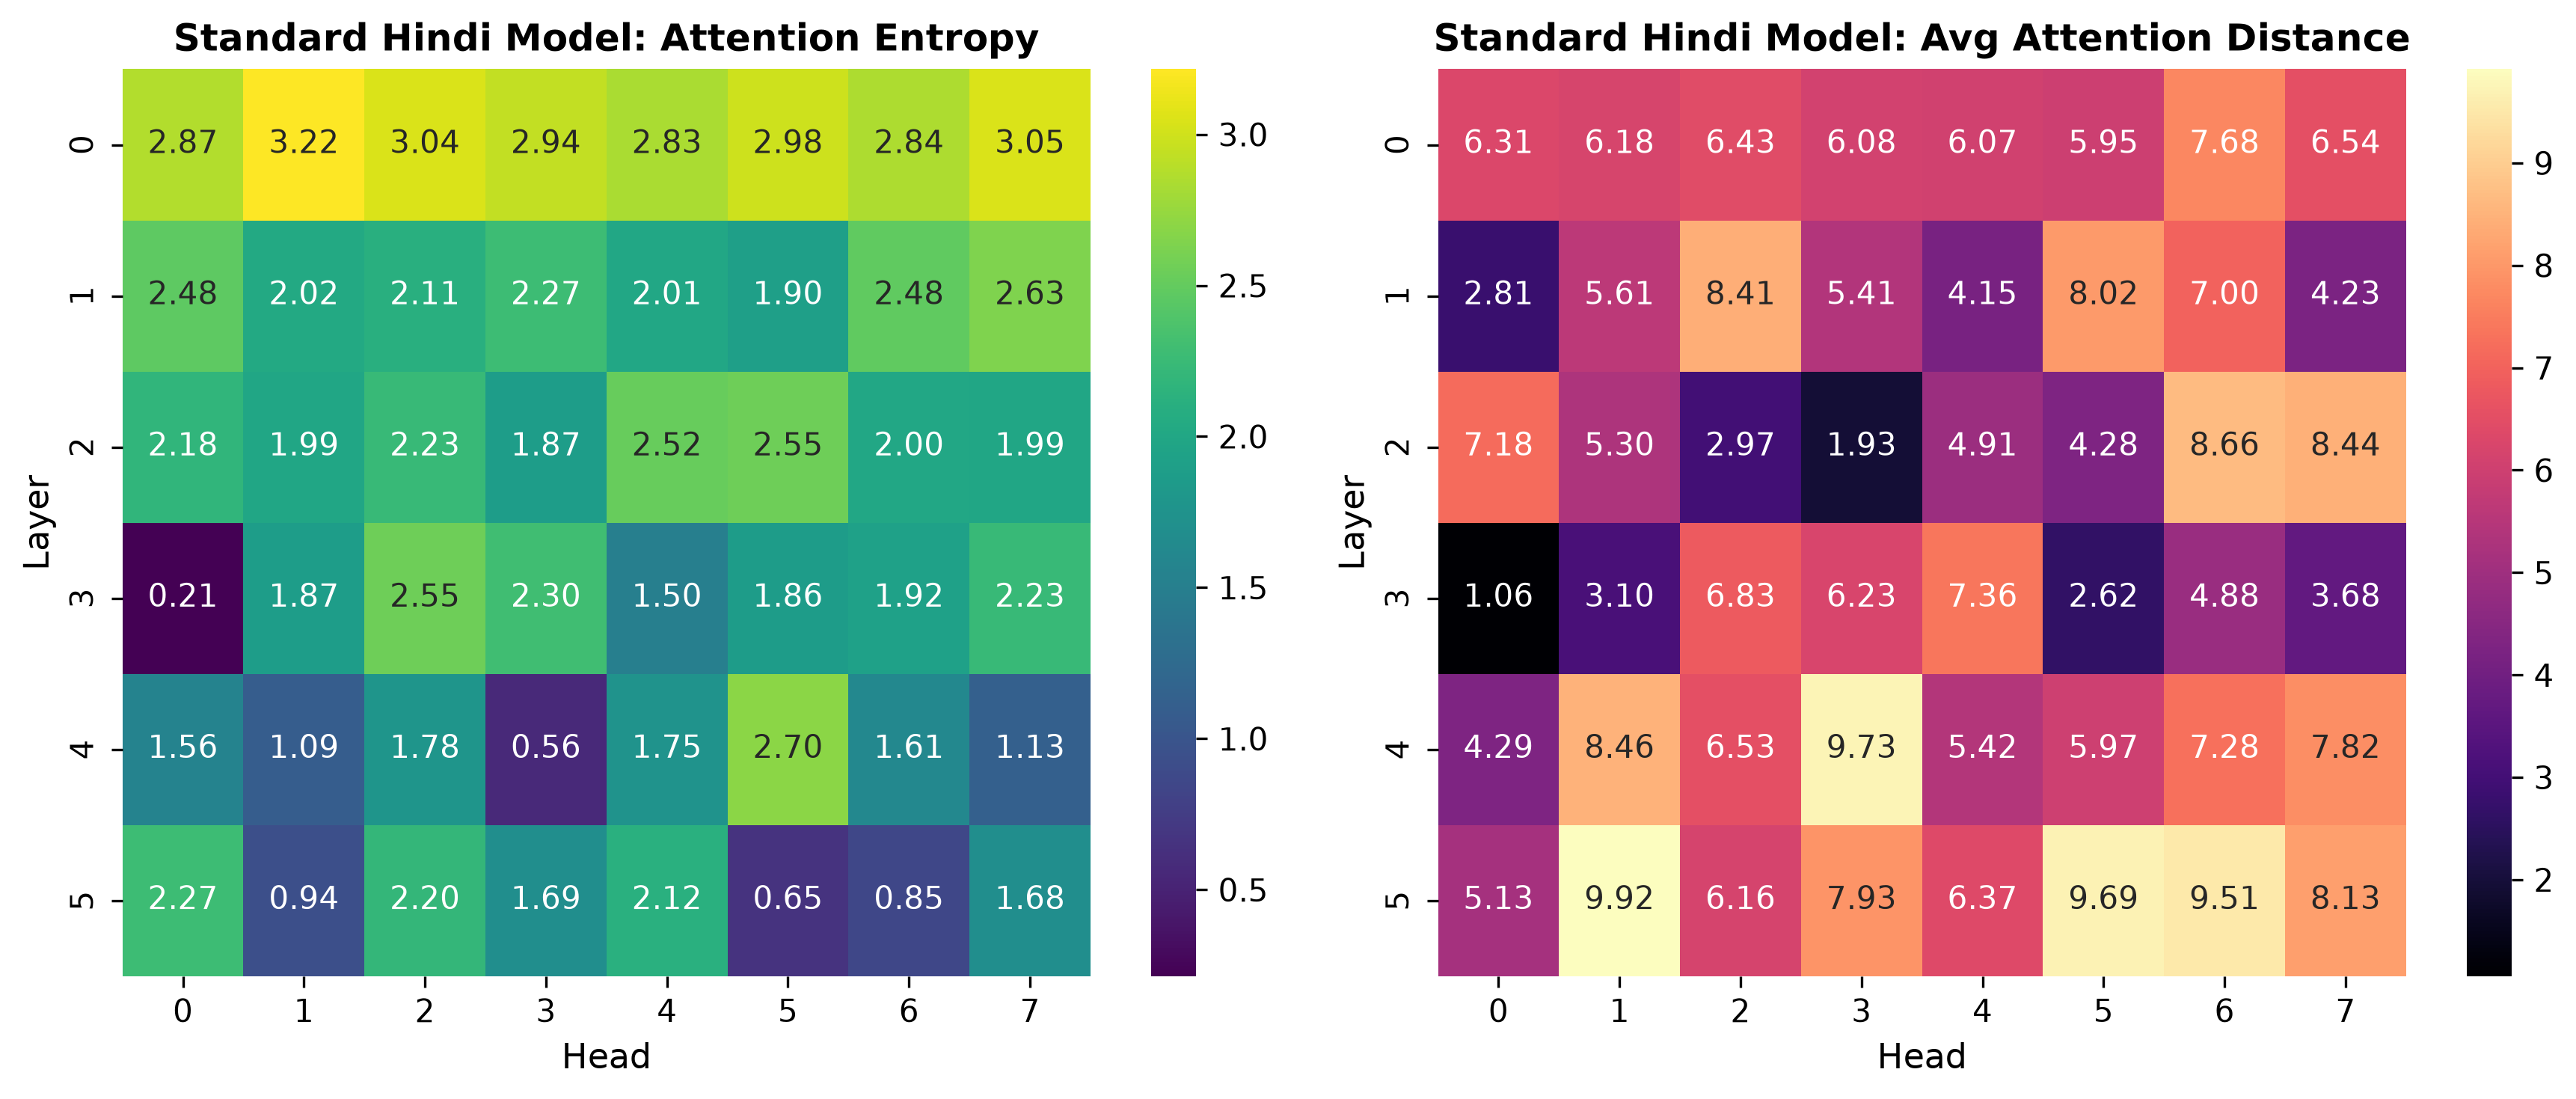
\includegraphics[width=0.95\textwidth]{plots/phase2_hindi_attn_entropy_distance.png}
\caption{Hindi attention entropy and mean attention distance across layers and heads. Early layers show low entropy, late layers show higher entropy and longer semantic context windows.}
\end{figure}

I also conducted an attention analysis on the Phase 2 base models to see how they process text. Looking closely at the attention weights showed that early layers (like Layer 0) focus heavily on immediate neighbors (concentrated diagonal attention). By the deeper layers (like Layer 5), the attention becomes much broader with a longer average attention distance, allowing the model to capture larger sentence-level semantic dependencies. I also verified causal masking fidelity: modifying the final input token produced strictly zero perturbation in prior hidden states. Having confirmed that both base models successfully internalized language syntax, I proceeded to Phase 3 to test structured deductive reasoning.

\clearpage
\section{Phase 3: Reasoning Finetuning}

\subsection{Synthetic Reasoning Dataset}

While the Phase 2 base models generate sentences that follow basic grammar rules, open-ended language models are prone to hallucination. In Phase 3, I investigated whether these 24M-parameter models could acquire systematic reasoning capabilities through supervised instruction finetuning. I built a script that generates complex relational and logical problems across both languages, ensuring that the Nepali generator was implemented with native morphology rather than mechanical translations of Hindi templates.

\begin{table}[htbp]
\centering
\caption{Reasoning dataset structure and task complexity tiers}
\begin{tabular}{lp{12.5cm}}
\toprule
\textbf{Tier} & \textbf{Task Focus and Problem Structure} \\
\midrule
Tier 1 & Direct numeric and attribute comparisons between two entities. \\
Tier 2 & Transitive chains (A > B > C), ranking, numeric threshold filtering, and difference calculations. \\
Tier 3 & Temporal sequence ordering, logical contradiction checks, rule classification, and conditional deduction. \\
\bottomrule
\end{tabular}
\end{table}

The dataset encompasses 13 distinct problem categories totaling 9,000 validated examples per language (split 70/15/15 into train/validation/test). I generated this data entirely from scratch using a Python script, combining 26 real-world attributes (like speed in km/h or price in rupees) with 53 different phrasing templates. Each training example was formatted as a prompt followed by \texttt{\textbackslash n Answer: answer}. To prevent data leakage, I used a fixed seed (\texttt{\_SPLIT\_SEED = 20260913}) to partition the entity pools before generating the text, meaning the models were tested on entities and phrasings they had genuinely never seen before.

\subsection{Finetuning Protocol and Loss}

I adapted each model by resuming training from its Phase 2 pretrained checkpoint while keeping the tokenizer frozen. I implemented selective loss masking by assigning a target label of -100 to all prompt tokens, ensuring that gradient updates backpropagate strictly through the generated answer tokens. Training proceeded for 3 epochs with AdamW ($5 \times 10^{-5}$, cosine decay). 

\begin{figure}[htbp]
\centering
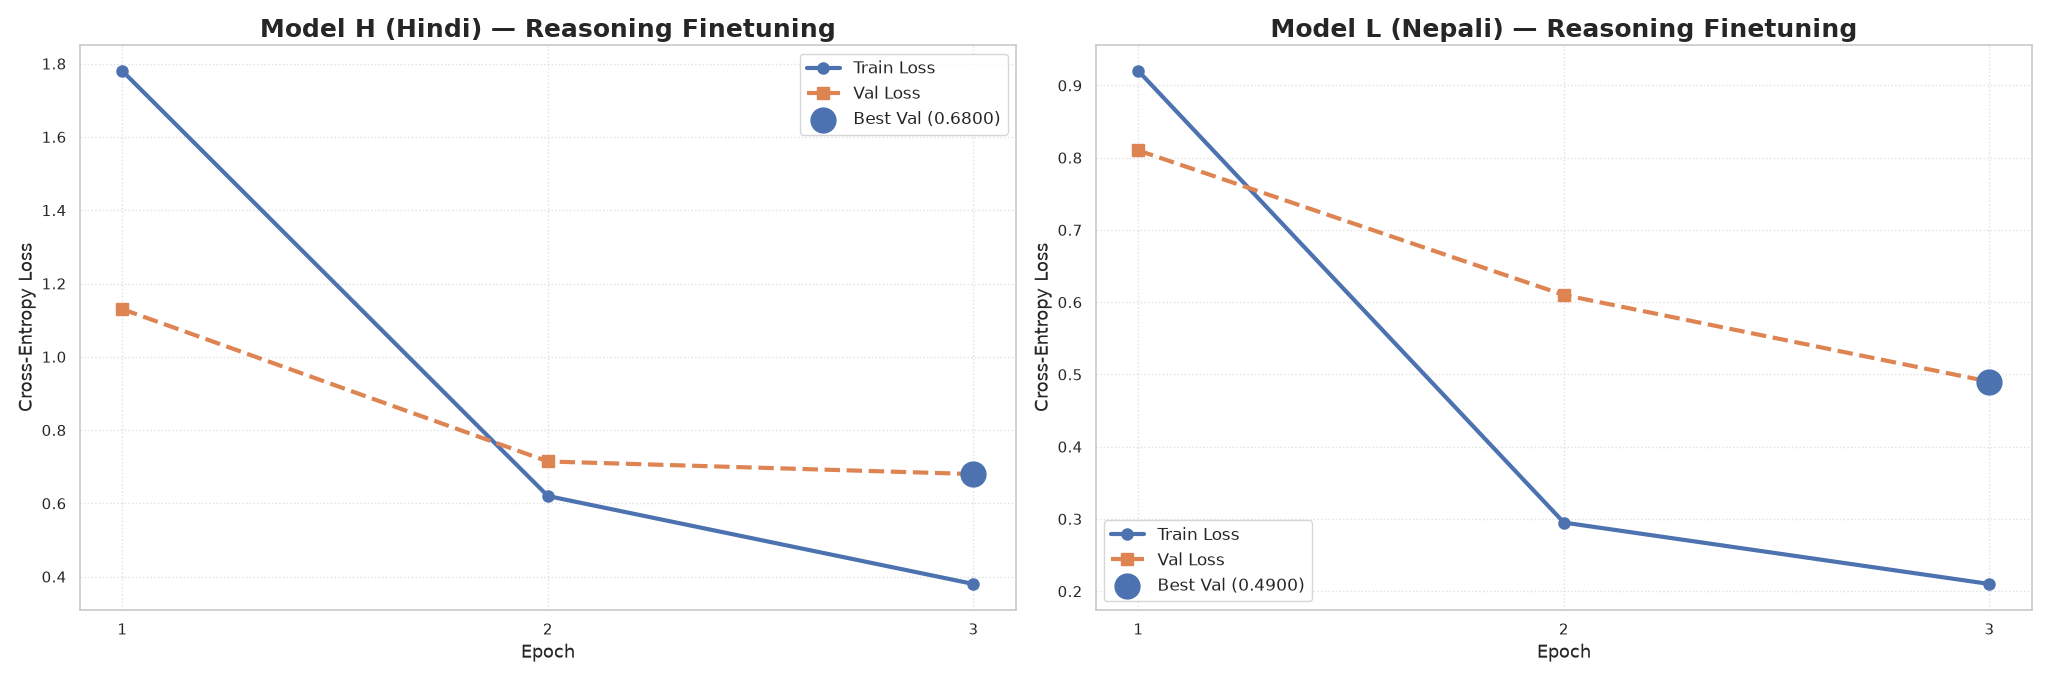
\includegraphics[width=0.9\textwidth]{plots/phase3_finetuning_loss_curves.png}
\caption{Finetuning loss curves. Hindi generalizes steadily while Nepali overfits after Epoch 1.}
\end{figure}

The resulting loss trajectories revealed a dramatic contrast between the two language pipelines. Hindi (Model H) displayed very stable training, so I selected its epoch 3 checkpoint. Nepali (Model L) began with a lower initial loss but quickly overfit, with validation loss hitting its minimum at epoch 1 and worsening thereafter. I selected its epoch 1 checkpoint. This overfitting is driven by a major difference in how the tokenizers work: Model L used a character-level BPE tokenizer, which fragments Nepali words into smaller, less semantically cohesive units compared to Hindi's byte-level BPE. Combined with a narrower pretraining corpus, Model L's base representations were not as well-developed, causing it to memorize synthetic templates rapidly rather than learning generalized logic.

\subsection{Reasoning Results and Analysis}

I evaluated the 1,350 held-out test prompts under greedy decoding. \textbf{Strict Exact Match} requires the entire generated text to match the gold target string identically, while \textbf{Substring Match} extracts the first generated sentence and verifies whether the gold entity is present.

\begin{table}[htbp]
\centering
\caption{Held-out reasoning accuracy across pretrained and finetuned models (percent)}
\begin{tabular}{p{6.1cm}rr}
\toprule
\textbf{Evaluation Metric} & \textbf{Hindi (Model H)} & \textbf{Nepali (Model L)} \\
\midrule
Pretrained strict exact match & 0.00\% & 0.00\% \\
Finetuned strict exact match & 0.00\% & 0.00\% \\
Pretrained substring match & 1.04\% & 1.93\% \\
Finetuned substring match & 27.26\% & 26.67\% \\
Tier 1 after finetuning & 38.98\% & 37.50\% \\
Tier 2 after finetuning & 18.50\% & 17.45\% \\
Tier 3 after finetuning & 31.95\% & 34.49\% \\
\bottomrule
\end{tabular}
\end{table}

Strict exact match is 0.00\% because target labels are short entity names, whereas the finetuned models learned to produce full, natural explanatory sentences. Because greedy decoding continues until the end-of-sequence token, full string matching is overly punitive. Substring matching provides a clearer picture:
\begin{itemize}
\item \textbf{Tier 1 (Pairwise Comparison):} The prompt mentions two candidate entities (a 50\% baseline). Model H achieves 38.98\% and Model L achieves 37.50\%, both falling below the naive 50\% copy baseline. 
\item \textbf{Tier 2 (Multi-Step Logic):} With 3 to 4 candidates in ranking tasks, the copy baseline is 25-33\%. The models score 18.50\% and 17.45\%, indicating that relational chains remain largely unlearned.
\item \textbf{Tier 3 (Rule Classification):} Scores rise to $\sim$32-34\%, driven by binary yes/no questions which inherently carry a 50\% prior.
\end{itemize}

When inspecting the outputs, I noticed three common failure modes:
\begin{enumerate}
\item \textbf{No stopping:} The model often correctly generated the entity but then kept writing a full sentence instead of stopping, which is why the strict exact match score is 0\%.
\item \textbf{Position bias:} On Tier 1 questions, it disproportionately guessed the entity that was mentioned last in the prompt, leading to scores below random chance.
\item \textbf{Chain collapse:} For 4-hop chain questions, it frequently guessed an entity from the middle of the chain rather than the extreme ends.
\end{enumerate}
Ultimately, finetuning taught the models how to format an answer and copy an entity, but it did not teach them actual logical reasoning. 

\begin{figure}[htbp]
\centering
\begin{subfigure}[b]{0.48\textwidth}
  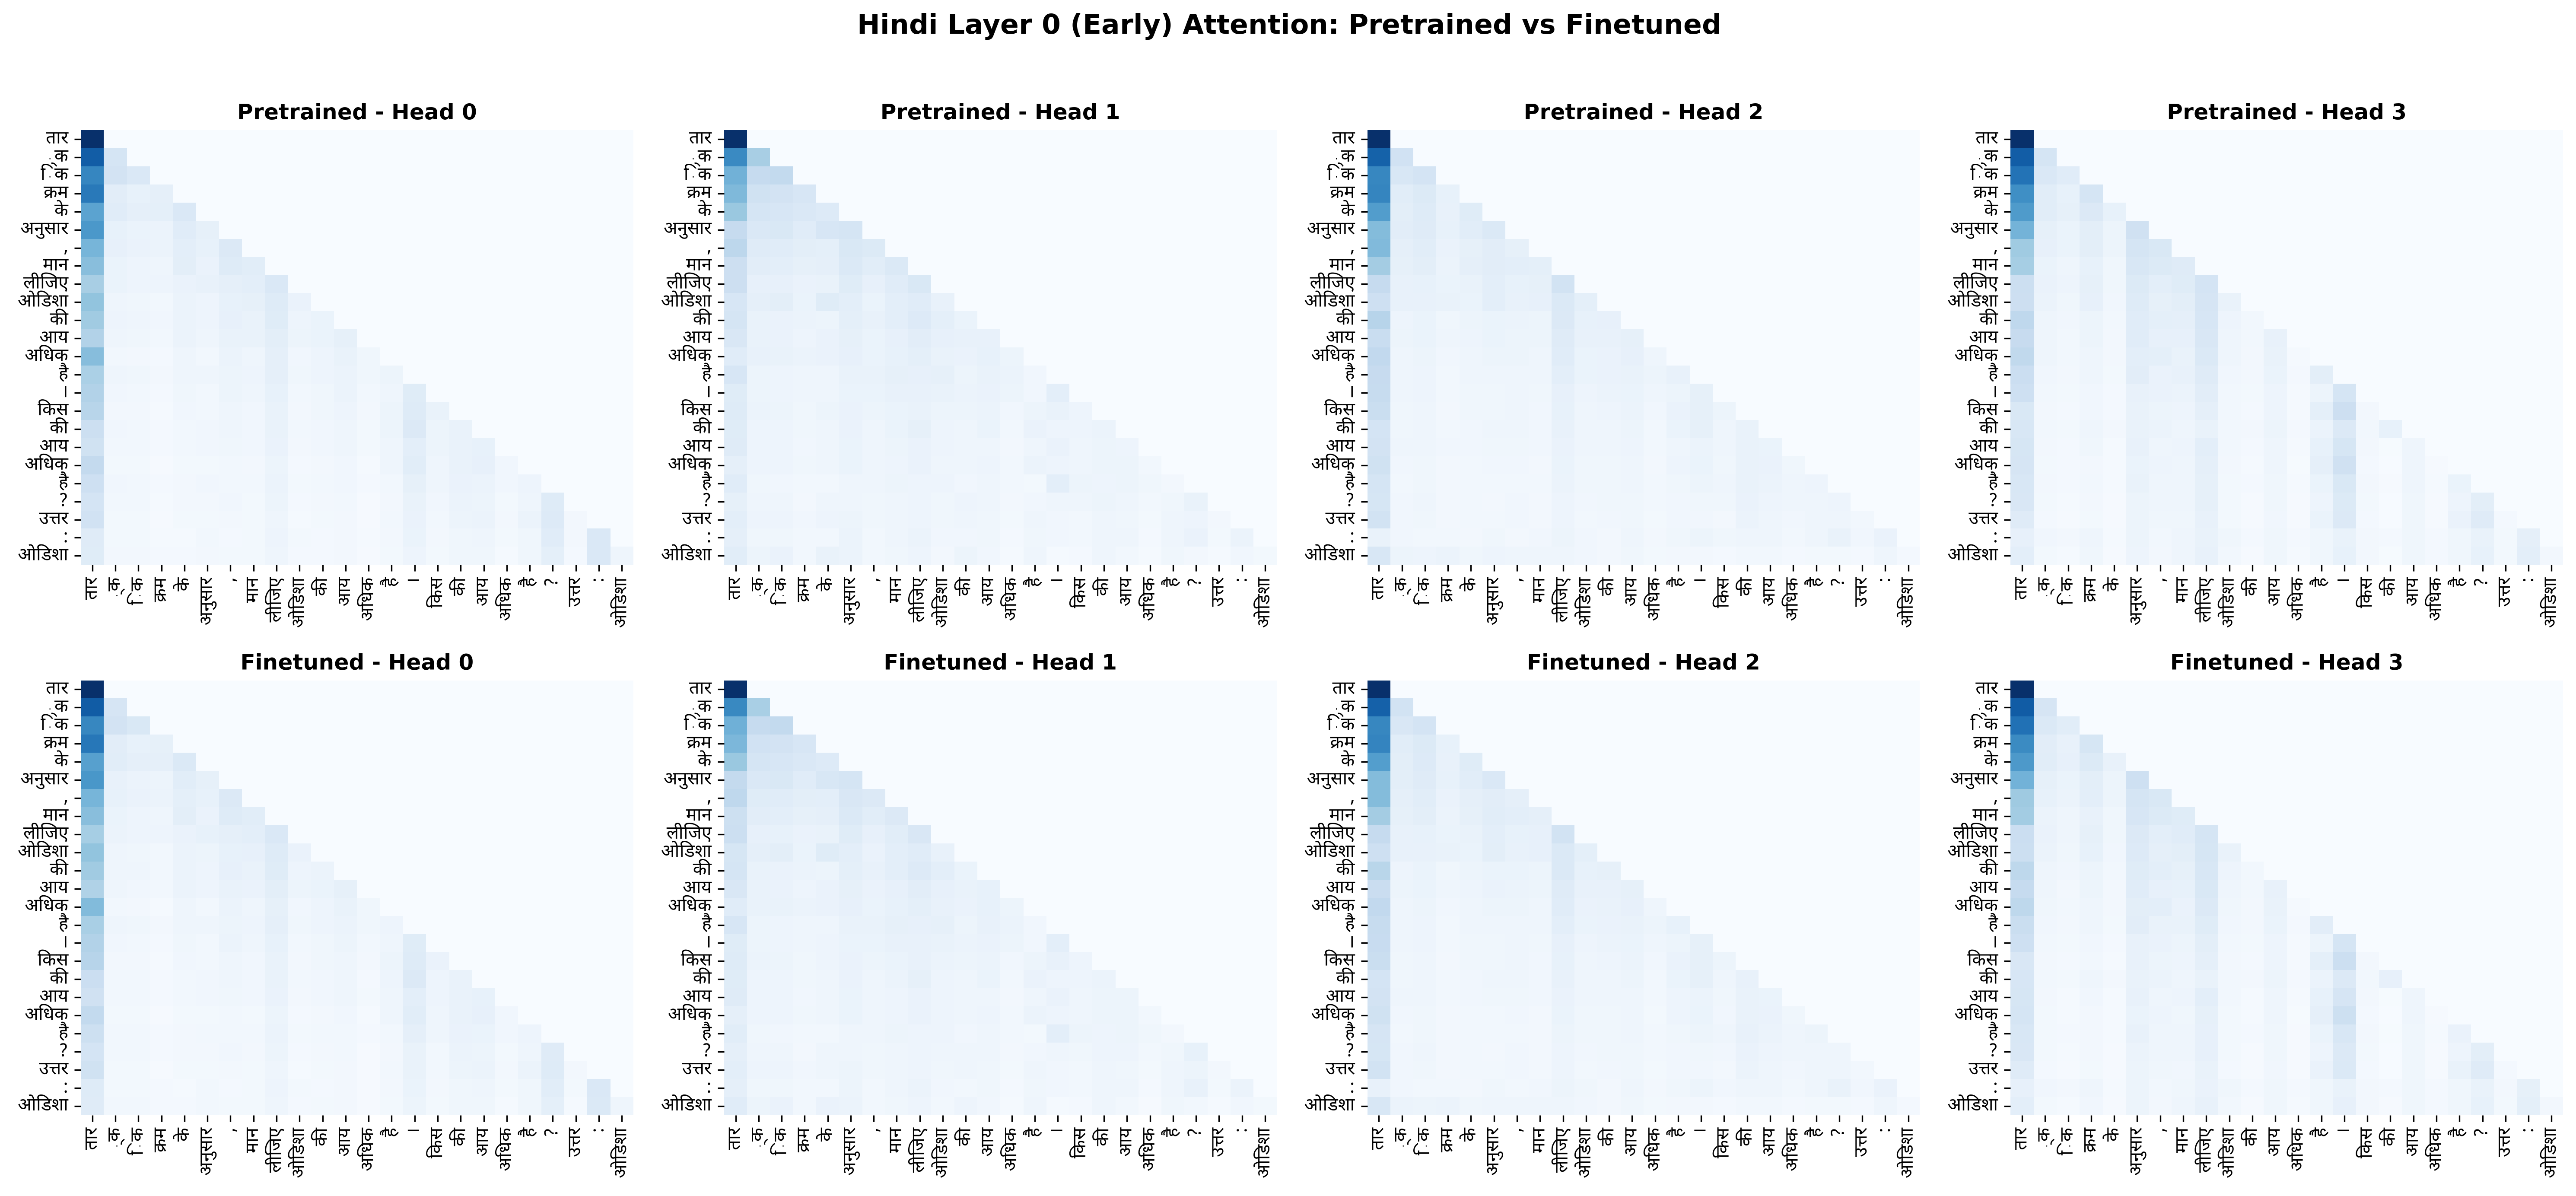
\includegraphics[width=\textwidth]{plots/phase3_hindi_attn_compare_layer0.png}
  \caption{Hindi Layer 0 (Early)}
\end{subfigure}
\hfill
\begin{subfigure}[b]{0.48\textwidth}
  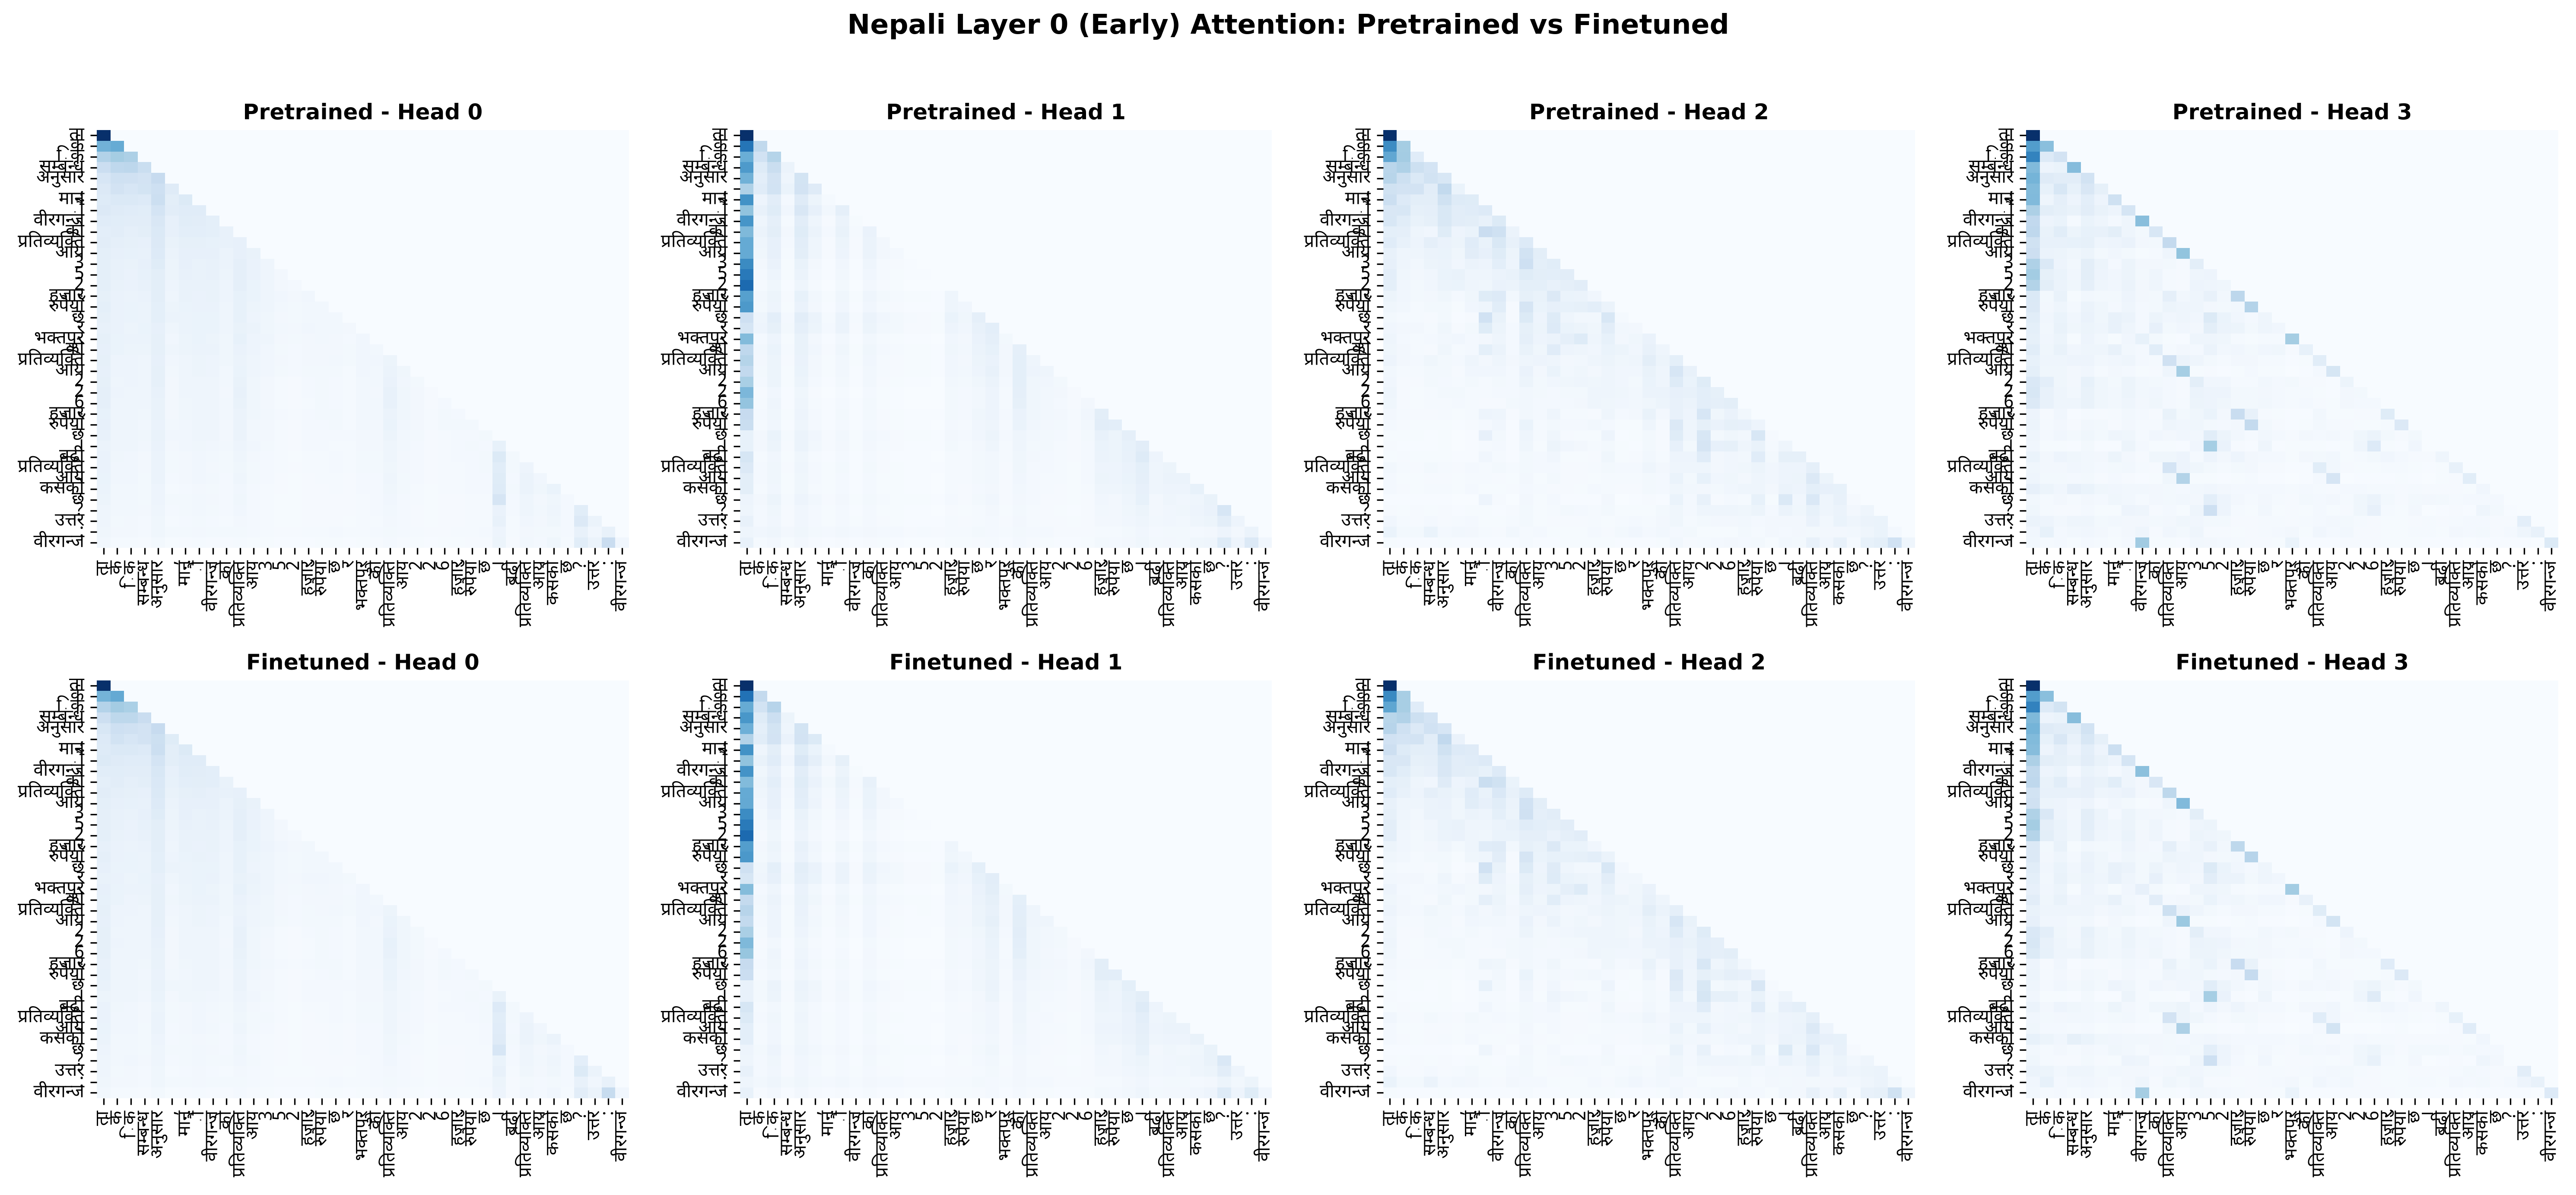
\includegraphics[width=\textwidth]{plots/phase3_nepali_attn_compare_layer0.png}
  \caption{Nepali Layer 0 (Early)}
\end{subfigure}
\vskip 8pt
\begin{subfigure}[b]{0.48\textwidth}
  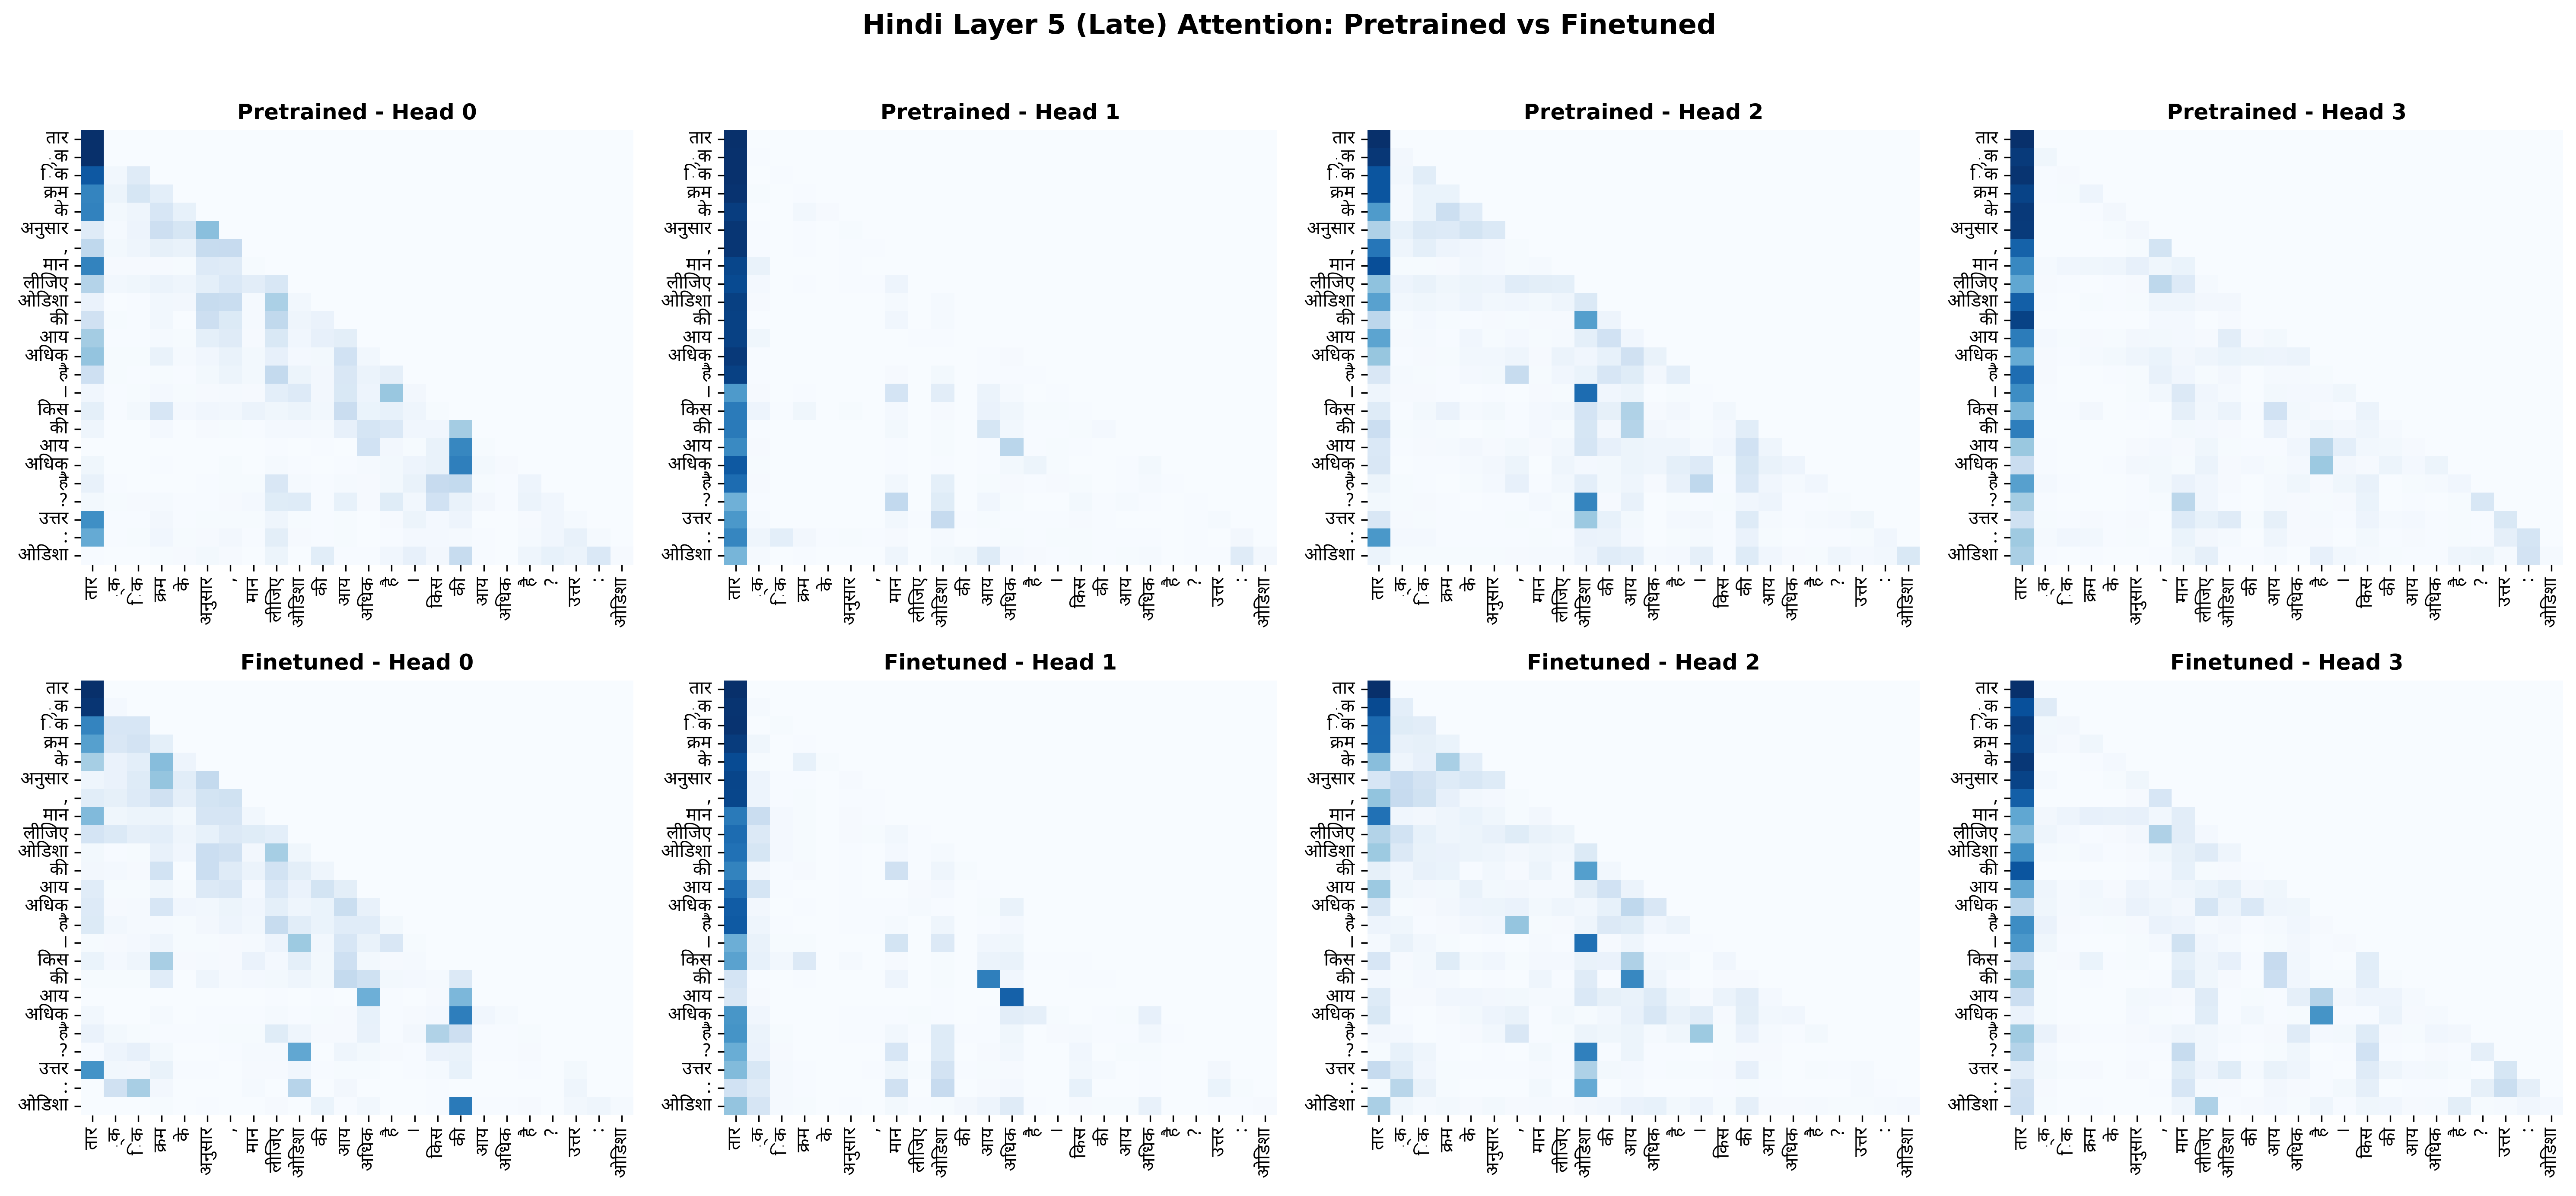
\includegraphics[width=\textwidth]{plots/phase3_hindi_attn_compare_layer5.png}
  \caption{Hindi Layer 5 (Late)}
\end{subfigure}
\hfill
\begin{subfigure}[b]{0.48\textwidth}
  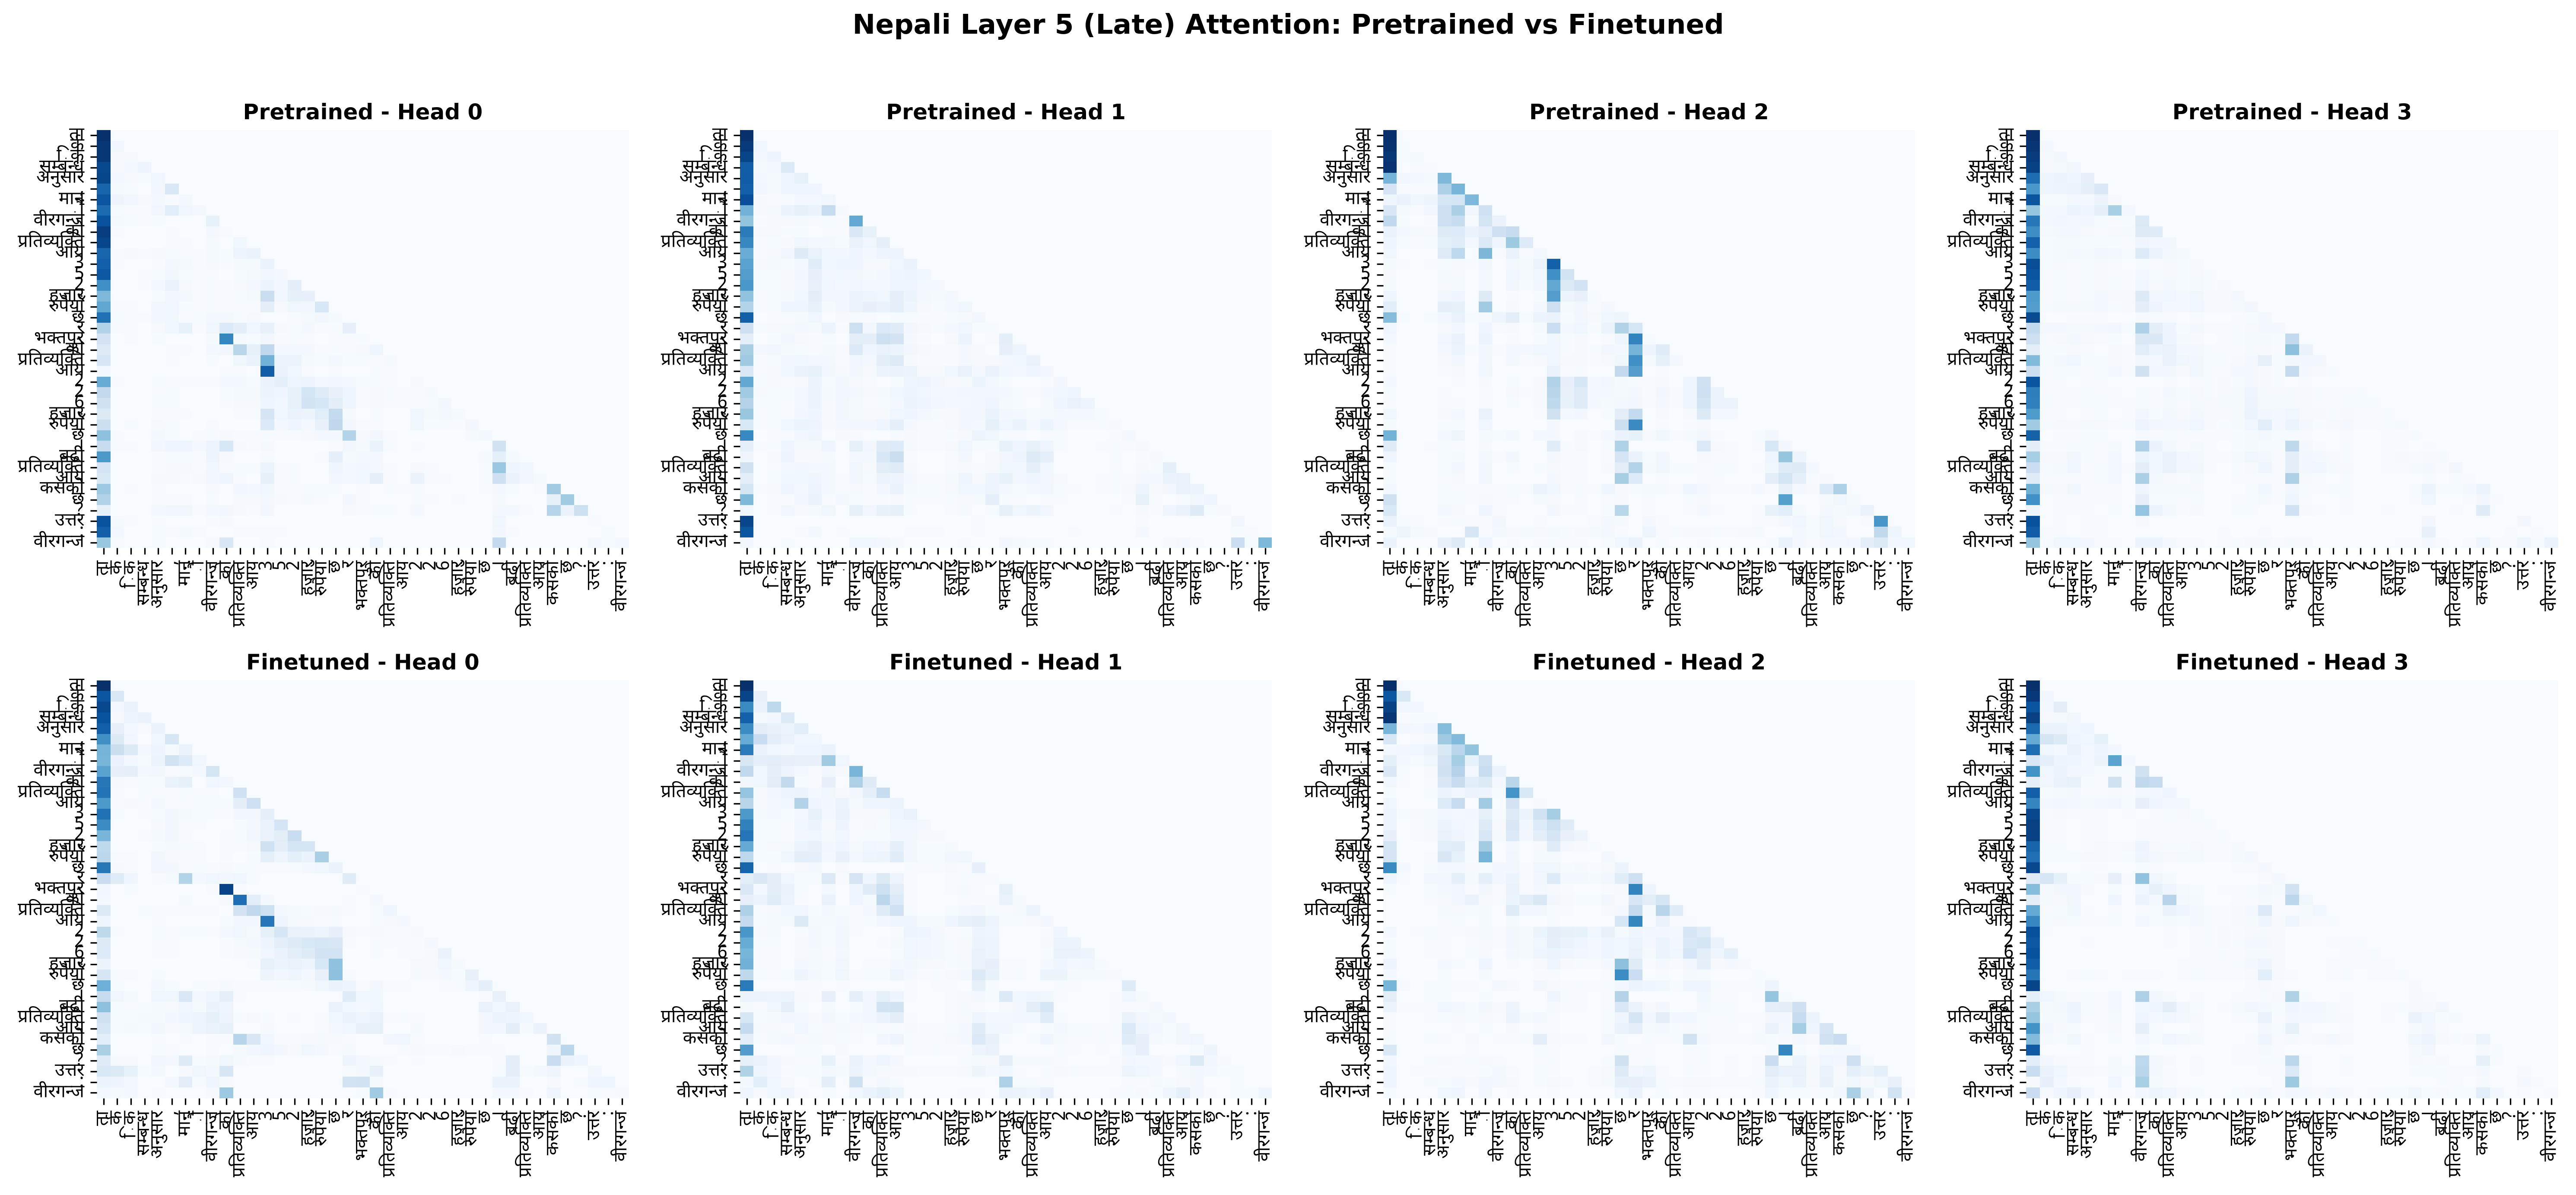
\includegraphics[width=\textwidth]{plots/phase3_nepali_attn_compare_layer5.png}
  \caption{Nepali Layer 5 (Late)}
\end{subfigure}
\caption{Attention maps before and after finetuning. Late layers develop sharp retrieval and copy circuits.}
\end{figure}

Looking at the attention maps before and after finetuning explains why this happens. The early layers (like Layer 0) barely changed, they kept their strong focus on immediate neighbors and the first token (an attention sink). However, the late layers changed significantly. For example, in Hindi Layer 5, Head 1 developed a sharp link between question words (like 'kis ki' [whose]) and the attribute noun (like 'aay' [income]), while Head 2 strengthened its focus on the target entity (like 'Odisha') to copy it into the answer. Nepali showed a similar pattern. Both models learned the format of where to copy the answer from, but lacked the capacity and data to actually learn the math or logic needed to pick the right entity.

\textbf{Final Project Comparison}
\textbf{1. Data scale and quality:} Hindi had an abundant multi-domain crawl. Nepali relied on a handful of news sites, meaning Model L's corpus was far narrower and more repetitive at the same token count.
\textbf{2. LM vs Reasoning results:} Nepali achieved better LM metrics (lower BPB), but this just reflects its repetitive, easier-to-predict corpus grading its own homework. On reasoning, they scored identically ($\sim$27\%) because the synthetic datasets were perfectly size-matched.
\textbf{3. Tokenizer factors:} The Nepali BPE learned longer tokens because of the repetitive corpus. This flatters BPB but fragments unseen test entities badly. Corpus diversity mattered more than the tokenizer itself.
\textbf{4. Evidence for differences:} The loss curves (Nepali overfits in 1 epoch), matched reasoning scores, and identical late-layer attention maps prove the differences stem entirely from the underlying data distributions and not the model architecture.

\clearpage
\section{Bonus: Positional Embedding Ablation}

We observed how attention heads rely on sequential structure to build syntactic and copy circuits. This raises a fundamental architectural question: Does causal masking alone supply sufficient sequential ordering, or are learned positional embeddings strictly absolutely necessary? To answer this, I conducted a full ablation study, retraining Model H from scratch for 61,036 steps with identical hyperparameters and compute budget, but with learned positional embeddings completely removed.

\begin{table}[htbp]
\centering
\caption{Standard Hindi Model H versus the No-Position Ablation model}
\begin{tabular}{p{5.5cm}rrr}
\toprule
\textbf{Evaluation Metric} & \textbf{Standard Model H} & \textbf{No-Position Ablation} & \textbf{Relative Change} \\
\midrule
Validation loss (nats) & 3.6487 & 4.0697 & +11.5\% \\
Perplexity (PPL) & 39.11 & 58.54 & +49.7\% \\
Bits per byte (BPB) & 0.5131 & 0.5674 & +10.6\% \\
4-gram repetition rate & 26.59\% & 68.52\% & +41.93 points \\
Distinct-1 vocabulary diversity & 0.4270 & 0.1703 & -60.1\% diversity \\
Mean attention distance & 7.15 tokens & 2.18 tokens & Collapsed to local \\
\bottomrule
\end{tabular}
\end{table}

\begin{figure}[htbp]
\centering
\begin{subfigure}[b]{0.48\textwidth}
  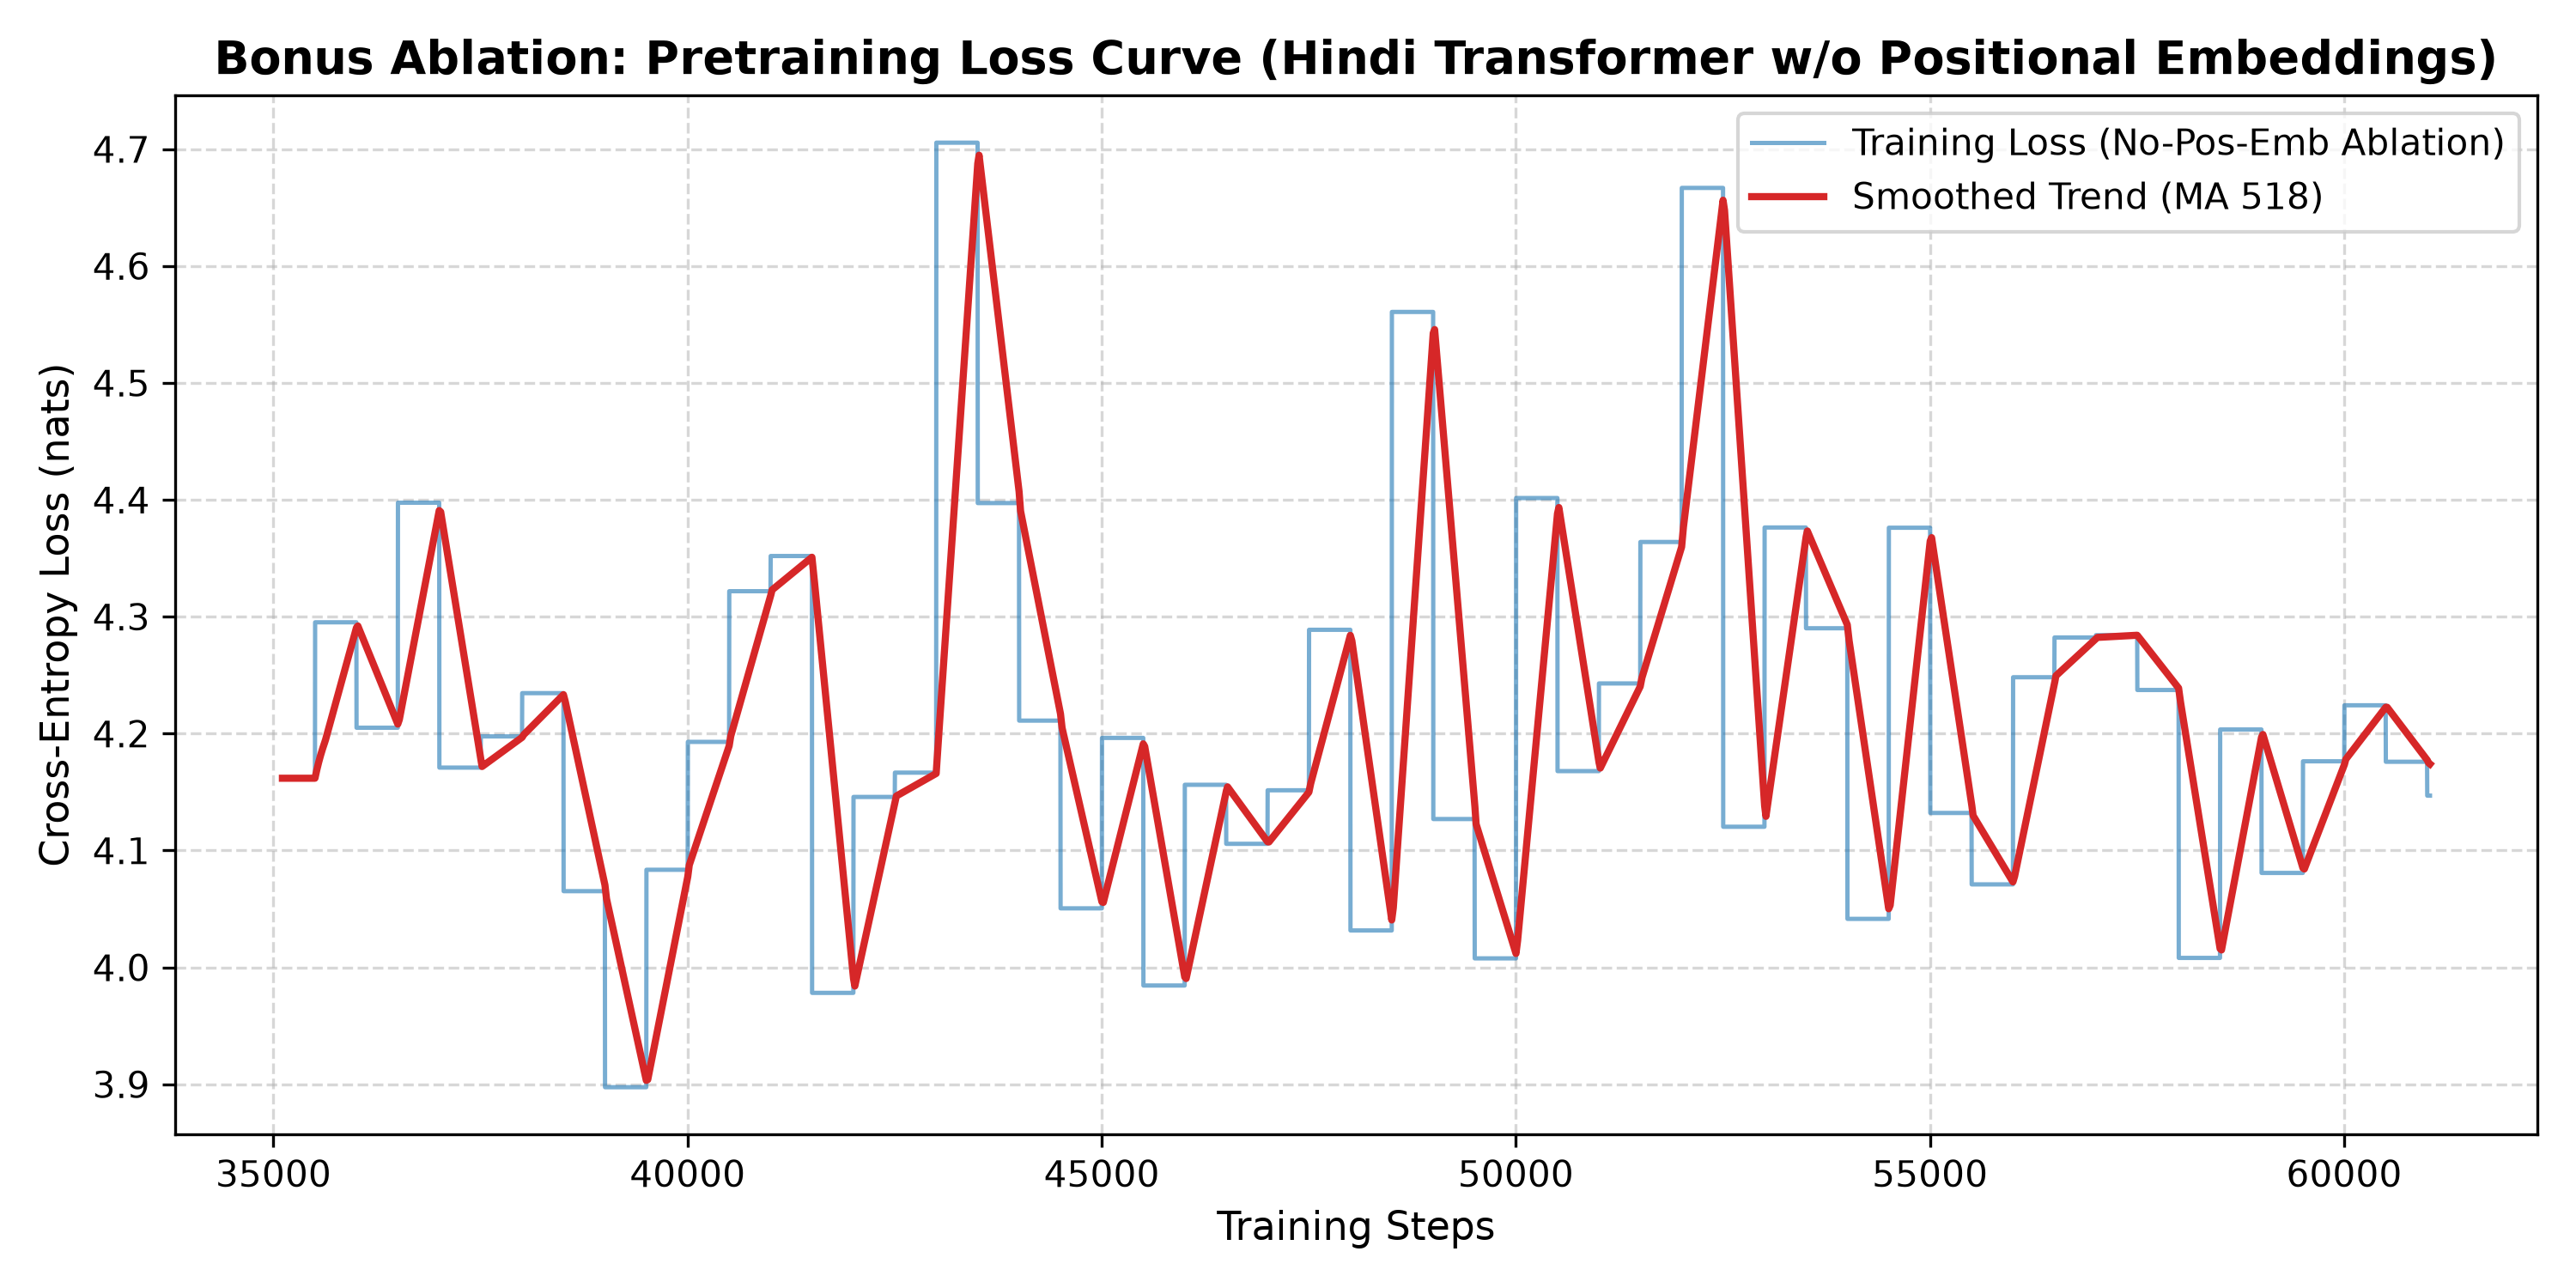
\includegraphics[width=\textwidth]{plots/bonus_ablation_loss_curve_smoothed.png}
  \caption{Training Loss}
\end{subfigure}
\hfill
\begin{subfigure}[b]{0.48\textwidth}
  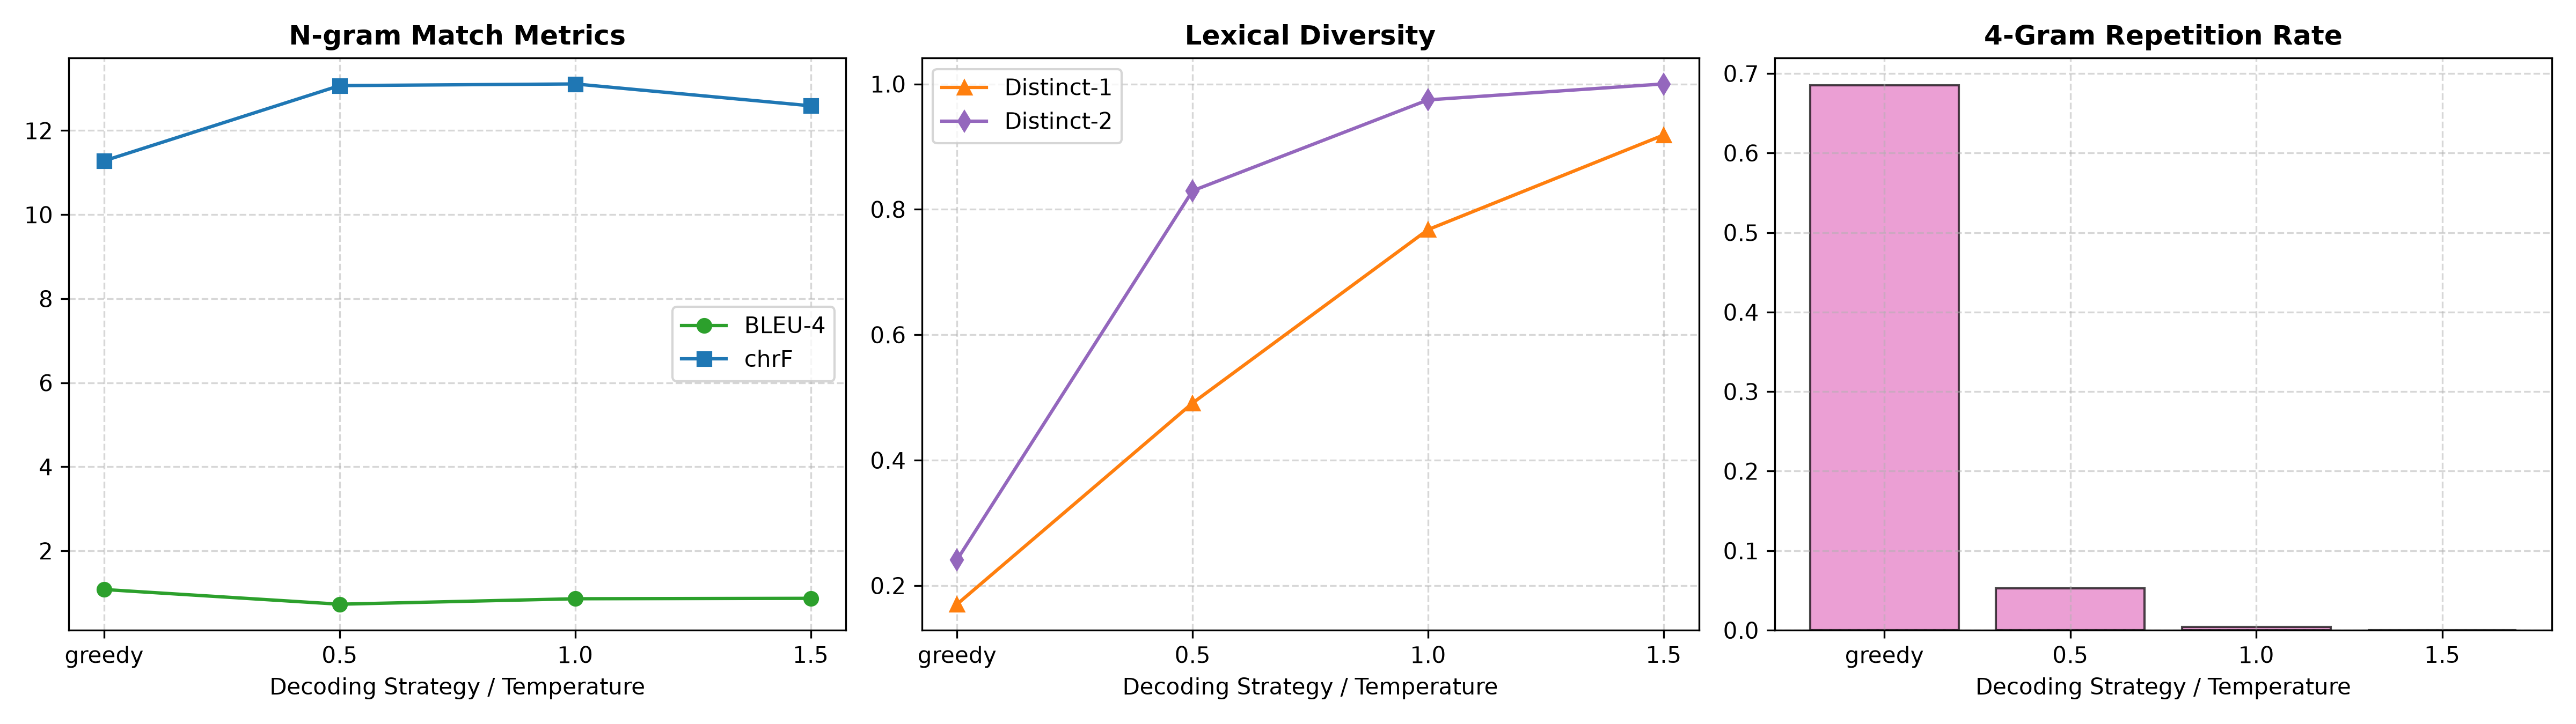
\includegraphics[width=\textwidth]{plots/bonus_ablation_generation_diversity.png}
  \caption{Generation Diversity}
\end{subfigure}
\caption{The ablated model plateaus at a higher loss and generates highly repetitive text.}
\end{figure}

The results demonstrate that positional embeddings are essential. Without positional inductive bias, the model suffers a 49.7\% spike in perplexity (39.11 to 58.54) and a severe collapse in generative diversity: 4-gram repetition skyrockets from 26.59\% to 68.52\%, while Distinct-1 drops from 0.4270 to 0.1703. While causal masking breaks the lack of sequence order by enforcing a lower-triangular visibility matrix, it cannot convey relative token distances, causing the Transformer to fail to understand sentence structure.

\begin{figure}[htbp]
\centering
\begin{subfigure}[b]{0.45\textwidth}
  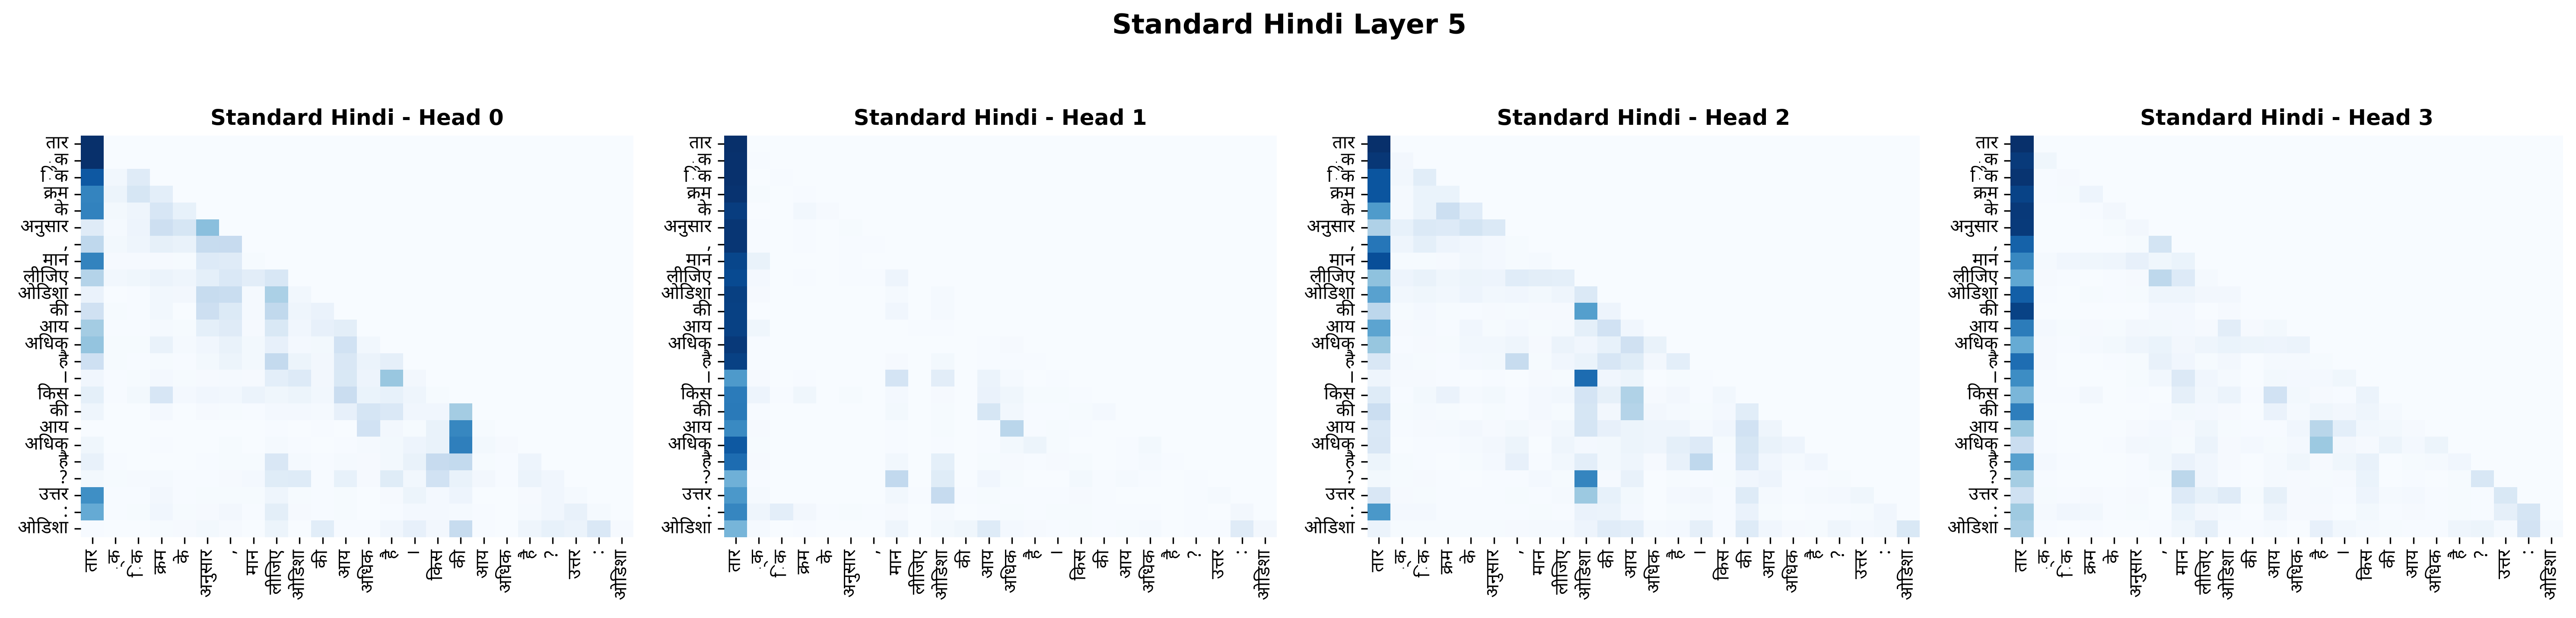
\includegraphics[width=\textwidth]{plots/phase2_hindi_attn_layer5.png}
  \caption{Standard Hindi: Layer 5}
\end{subfigure}
\hfill
\begin{subfigure}[b]{0.45\textwidth}
  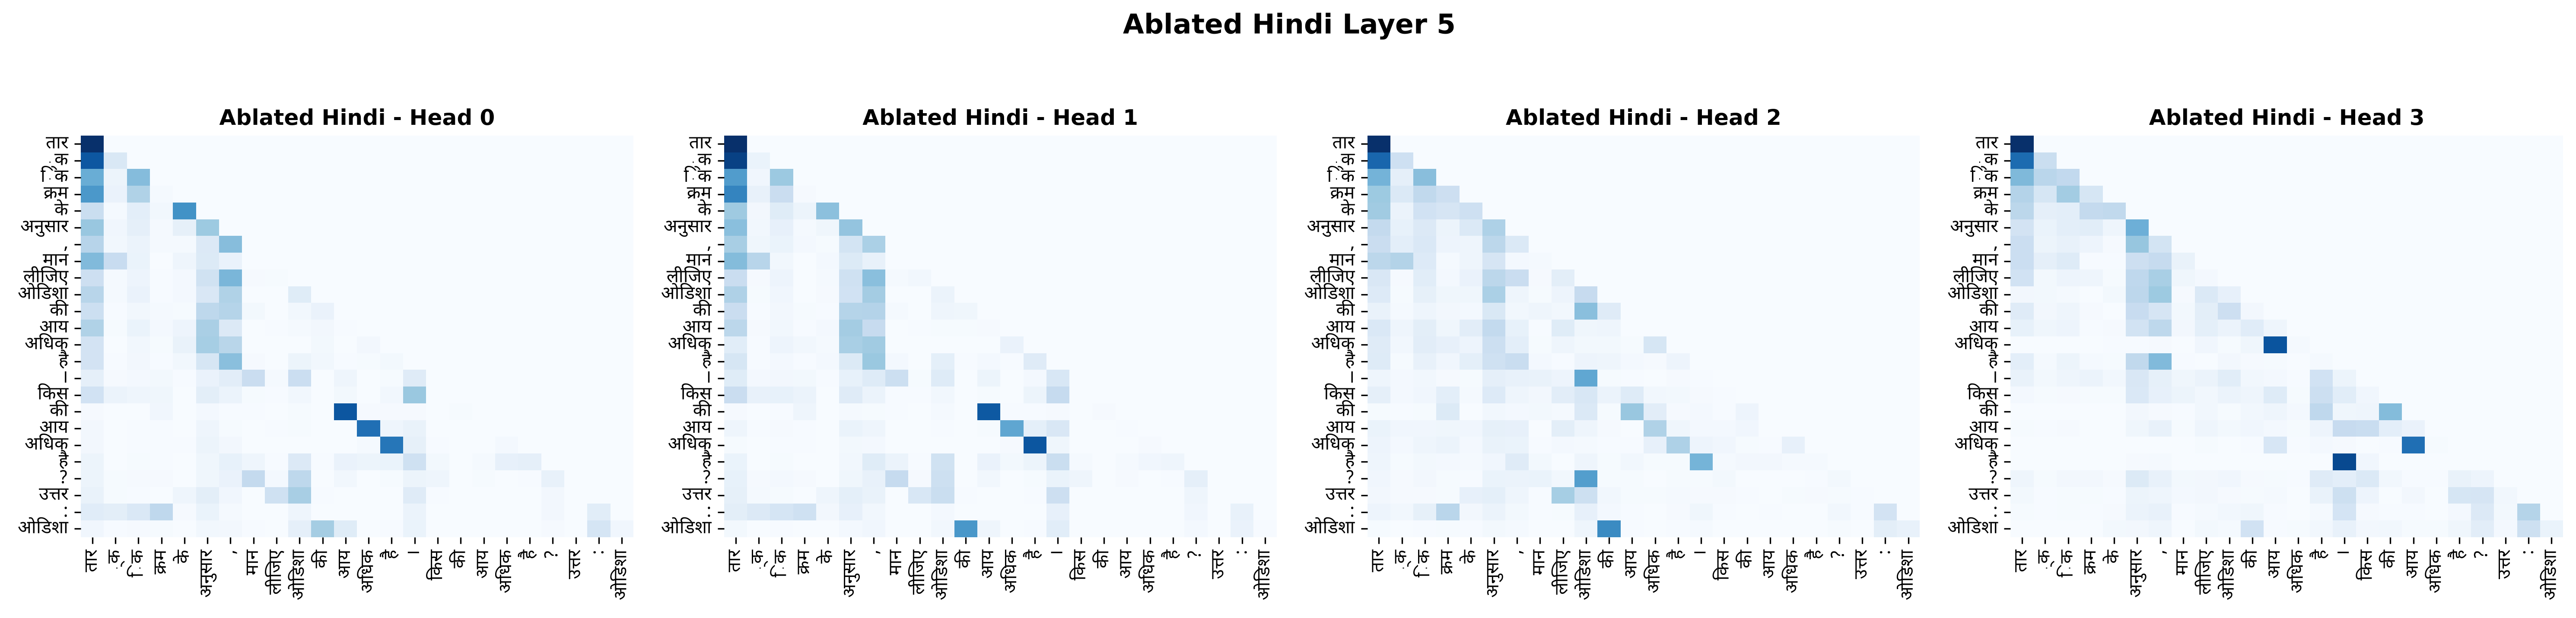
\includegraphics[width=\textwidth]{plots/bonus_ablation_attn_layer5.png}
  \caption{Ablated Hindi: Layer 5}
\end{subfigure}
\caption{Attention patterns. The ablated model collapses into a self-attending diagonal identity mapping.}
\end{figure}

\begin{figure}[htbp]
\centering
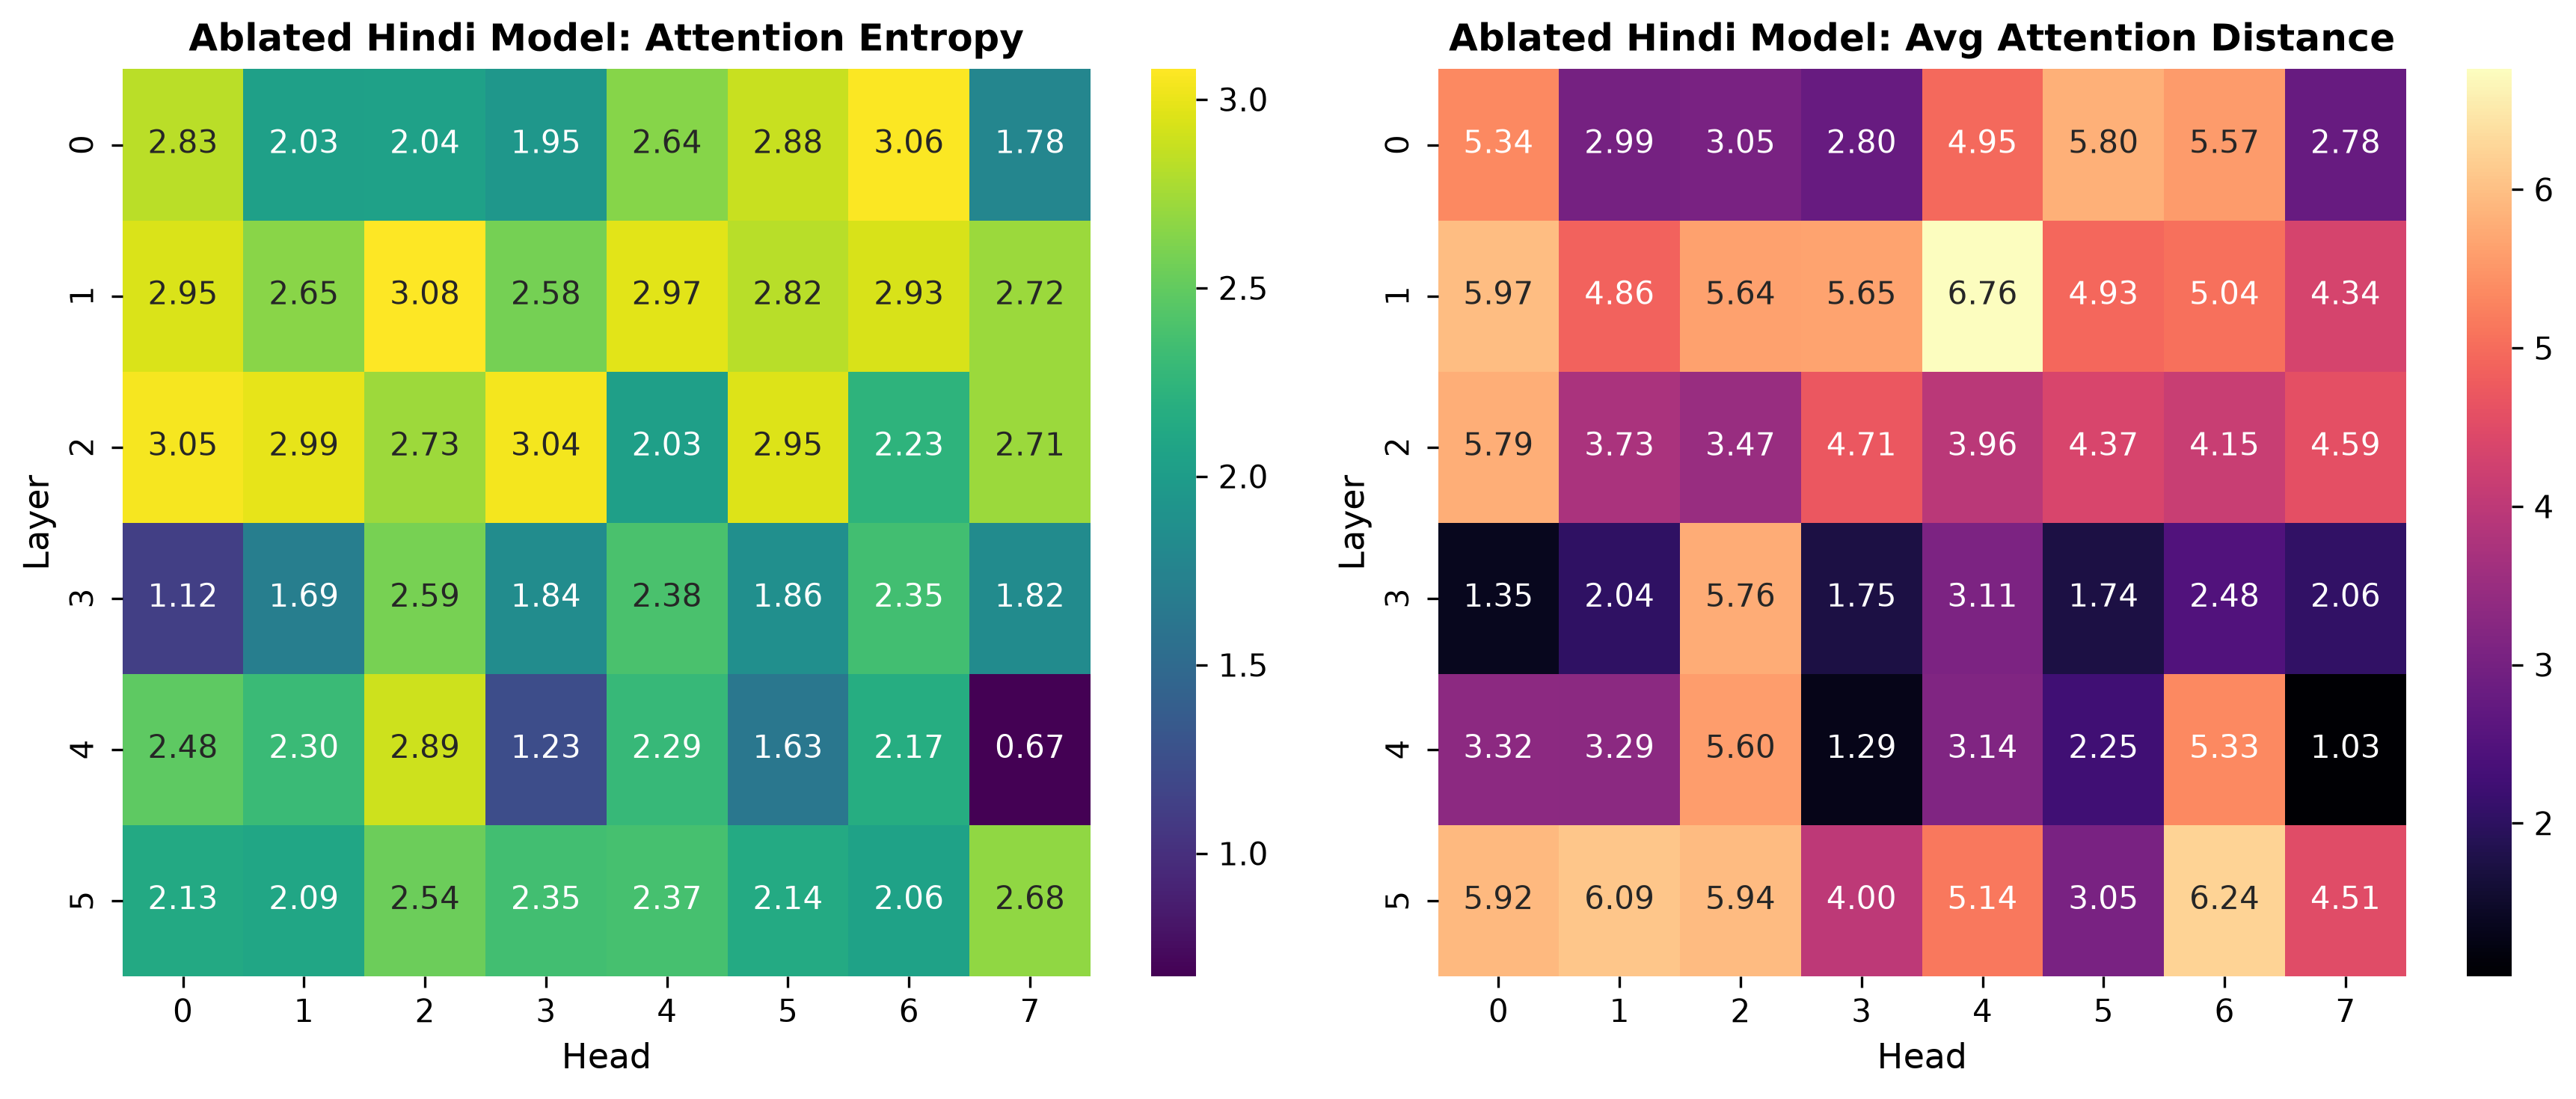
\includegraphics[width=0.85\textwidth]{plots/bonus_ablation_attn_entropy_distance.png}
\caption{Ablated model attention entropy and distance. The metrics are flat across all layers.}
\end{figure}

The standard model exhibits distinct layer-wise functional specialization, with low-entropy local attention in early layers and higher-entropy long-range attention in later layers. The ablated model is completely flat across all layers. Mean attention distance collapses from 7.15 down to 2.18. This proves that the attention mechanism cannot organize itself without position information to anchor heads to, confirming that positional embeddings are absolutely necessary for Transformer language modeling.

\textbf{Hypothesis vs. Findings.} The theoretical expectation was that self-attention, being essentially a set-operation, would fail completely to learn syntax without positional embeddings. However, I hypothesized that causal masking which inherently provides the model with a basic sense of "past" versus "future" might provide just enough sequential bias for the model to generate somewhat coherent short phrases.

Our findings ultimately reject this hypothesis and strongly confirm the theoretical expectation. While causal masking breaks perfect sequence invariance, the severe spike in perplexity (from 39.11 to 58.54) and the dramatic collapse in vocabulary diversity prove it is not enough to build long-range syntactic dependencies. As shown by the attention distance dropping to 2.18 tokens, the ablated model devolved into looking only at its immediate neighbors, functioning like a basic local bag-of-words. It completely lost the layer-wise specialization seen in Phase 2 (where deeper layers look further back in the sentence). This confirms that while causal masking creates a one-way street for information flow, explicit positional embeddings are absolutely required for the attention mechanism to learn structure and syntax.

\end{document}
